\documentclass[10pt]{report}

\usepackage{template}
\usepackage[backend=biber,style=alphabetic]{biblatex}
\addbibresource{bibliography.bib}

\newglossaryentry{graph}{
    name=graph,
    description={- a set of nodes connected by edges}
}





\nomenclature[aaaaa]{$G$}{Graph}
\nomenclature[aaaba]{$\mathcal{G}$}{Set of all graphs}
\nomenclature[aabaa]{$V\br{G}$}{Set of vertices of $G$}
\nomenclature[aacaa]{$E\br{G}$}{Set of edges of $E$}
\nomenclature[aadaa]{$T$}{Tree}
\nomenclature[aadba]{$u\prec v$}{Vertex $u$ is a descendant of $v$}
\nomenclature[aadca]{$r\br{T}$}{Root of tree $T$}
\nomenclature[aadda]{$p_T\br{v}$}{Parent of $v$ in tree $T$}
\nomenclature[aadea]{$\mathcal{C}_T\br{v}$}{Children of $v$ in tree $T$}
\nomenclature[aadfa]{$T_v$}{Tree induced in $T$ by $v$ and all its descendants}
\nomenclature[aaeaa]{$F$}{Forest}
\nomenclature[aafaa]{$P$}{Path}
\nomenclature[aagaa]{$n\br{G}$}{Number of vertices of graph $G$}
\nomenclature[aahaa]{$m\br{G}$}{Number of edges of graph $G$}
\nomenclature[aaiaa]{$e=uv$}{Edge}
\nomenclature[aaiba]{$G[V']$}{Graph induced by $V'$ in $G$}
\nomenclature[aaica]{$G-v$}{Set of connected components after removal of $v$ from $G$}
\nomenclature[aaica]{$G-V'$}{Set of connected components after removal of $V'$ from $G$}
\nomenclature[aajba]{$N_G\br{v}$}{Set of neighbors of $v$ in $G$}
\nomenclature[aajca]{$N_G\br{V'}$}{Set of neighbors of the set $V'$ in $G$}
\nomenclature[aajaa]{$\deg_{G}\br{v}$}{Degree of vertex $v$ in $G$}
\nomenclature[aakaa]{$\Delta\br{G}$}{Degree of graph $G$}
\nomenclature[aalaa]{$P_T\br{u,v}$}{Path between $u$ and $v$ in tree $T$ (excl. $u,v$)}
\nomenclature[aamaa]{$P_T\br{V_1,V_2}$}{Path between $V_1$ and $V_2$ in tree $T$ (excl. $V_1,V_2$)}
\nomenclature[aanaa]{$T\angl{V'}$}{Minimal subtree of $T$ containing $V'$}
\nomenclature[aaoaa]{$\preceq$}{Partial ordering}
\nomenclature[aapaa]{$\mathcal{P}$}{Poset}
\nomenclature[aaqaa]{$c:X\to \mathbb{R}^+$}{Cost function (for general input $X$)}
\nomenclature[aaraa]{$w:X\to \mathbb{R}^+$}{Weight function (for general input $X$)}
\nomenclature[aarba]{$W:\mathcal{G}\to \mathbb{R}^+$}{Sum of weights in a graph}
\nomenclature[aasaa]{$s^*$}{Optimal solution}
\nomenclature[aatba]{$\OPT\br{I}$}{Cost of the optimal solution of the instance $I$}
\nomenclature[aauaa]{$\alpha \br{n}$}{Approximation factor}
\nomenclature[aavaa]{$q$}{Query}
\nomenclature[aavba]{$x$}{Target Vertex}
\nomenclature[aawaa]{$D$}{Decision tree}
\nomenclature[aaxaa]{$\mathcal{D}$}{Set of all decision trees}
\nomenclature[aayaa]{$C:\mathcal{D}, V \to \mathbb{R}^+$}{Cost of searching for a vertex}
   

% Custom title page commands
\newcommand{\supervisor}{prof. dr. hab. inż. Dariusz Dereniowski}
\newcommand{\university}{Faculty of Electronics, Telecommunications and Informatics\\Gdańsk University of Technology, Poland}
\newcommand{\theauthor}{Michał Szyfelbein}
\newcommand{\thetitle}{Experimental Analysis of Binary Search Models in Graphs}
\begin{document}
\usetikzlibrary {graphs,graphdrawing} \usegdlibrary {trees, layered, force}

\begin{titlepage}
    \centering
    \vspace*{2.5cm}
    {\Large\MakeUppercase{\university} \par}
    \vspace{3cm}
    {\Huge\bfseries\thetitle\par}
    \vspace{3cm}
    {\LARGE\theauthor \par}
    \vspace{1.5cm}
    {\large Supervisor: \supervisor \par}
    \vfill
    {\large \today}
\end{titlepage}

\chapter*{Abstract}

In this work, we conduct an experimental analysis of the generalized binary search problem in graphs. 
The analysis explores various classes of graphs, including: paths, trees and general graphs. The study is structured into two main sections:

The first part focuses on the theoretical foundations of the problem. It introduces key definitions, fundamental concepts, and pseudocodes of the analyzed procedures, along with a formal analysis of their parameters. The significance of these results was evaluated based on two primary metrics: the computational complexity and theoretical bounds on the quality of the solutions obtained.

The second part provides experimental verification of the theoretical claims established in the previous chapters. It also presents a practical comparison of the algorithmic approaches developed for different problem variants. The proposed procedures were evaluated across diverse graph classes thus ensuring complete results. To guarantee thorough and unbiased coverage of the problem space, all of the test instances were generated using randomized techniques and multiple input sizes were tested.

\paragraph{Keywords and phrases} Trees, Graph Searching, Binary Search, Decision Trees, Ranking Colorings, Graph
Theory, Approximation Algorithm, Combinatorial Optimization, Experimental Analysis of Algorithms


\singlespacing
\printnomenclature[0.5\textwidth]

\printglossaries

\tableofcontents
\listoffigures
\listoftables

\begin{frame}{Basic information}
	\textbf{The aim:} Experimental analysis of selected generalized binary search problems. The aim of the analysis is to verify the hypotheses regarding the effectiveness of search algorithms. 
    
    \textbf{Schedule:}
    \begin{itemize}
    \pause
    \item 2024.01 -- 2024.06: Researching and selection of the query model.
    \item 2024.06 -- 2025.05: Development and formal analysis of the proposed algorithms.
    \item 2025.06 -- 2025.10: Selection of models and algorithms for comparison, implementation, thesis writing.
    \item 2025.11 -- 2025.12: execution of experiments, analysis and interpretation of the results, finalization of the thesis.

\end{itemize}
\end{frame}

\begin{frame}{State of the work}
    \begin{itemize}
        \item Implementation, about 60\% complete:
        \begin{itemize}
        \item Language: \textbf{python},
        \item Libraries: \textbf{networkx},
        \item Environment: \textbf{PyCharm},
        \item Versioning: \textbf{git} + \textbf{github}, \hyperlink{https://github.com/MSzyfel/Binary-Search}{https://github.com/MSzyfel/Binary-Search}.
        \end{itemize} 
        \pause
        \item Thesis, about 80\% complete:
        \begin{itemize}
            \item Language: \textbf{LaTeX},
            \item Environment: \textbf{Visual Studio Code},
            \item Versioning: \textbf{git} + \textbf{github}, \hyperlink{https://github.com/MSzyfel/Papers}{https://github.com/MSzyfel/Papers}.
        \end{itemize} 
        \pause
        \item What is left: 
        \begin{itemize}
            \item Experiments,
            \item Advanced data generation,
            \item Optimization,
            \item Bug fixing,
            \item Data visualization.
        \end{itemize} 
    \end{itemize}
\end{frame}
\begin{frame}{Binary Search}
    
\begin{figure}[ht]
\centering
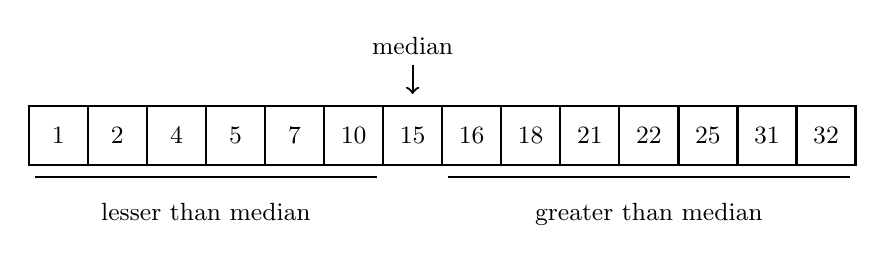
\begin{tikzpicture}[every node/.style={font=\small}, scale=0.75]

% --- Array values (10 elements) ---
\def\A{{1, 2, 4, 5, 7, 10, 15, 16, 18, 21, 22, 25, 31, 32}}
\def\MID{6} % Index of median (0-based): value = 23
% Draw array elements and indices
\foreach \i in {0,...,13} {
    \pgfmathsetmacro{\val}{\A[\i]}
    \draw[thick] (\i, 0) rectangle ++(1,1);
    \node at (\i+0.5, 0.5) {\val};
}

% Underline LEFT subarray (0..3)
\draw[thick] (0.1, -0.2) -- (6.0-0.1, -0.2);
% Label
\node[below=6pt] at (3, -0.2) {lesser than median};

% Underline RIGHT subarray (5..9)
\draw[thick] (7+0.1, -0.2) -- (13+1-0.1, -0.2);
% Label
\node[below=6pt] at (10.5, -0.2) {greater than median};

% Arrow for mid
\draw[<-, thick] (\MID+0.5, 1.2) -- +(0, 0.5) node[above] {median};

\end{tikzpicture}
\caption[Binary search]{Example of a sorted array containing 14 elements. }
\label{fig:binary-search-subarrays}
\end{figure}

\end{frame}


\begin{frame}{Generalized binary search}
        \begin{definition} A \textbf{searcher} is required to find a hidden \textbf{target} vertex $x$ in a graph $G$. To do so, they iteratively perform \textbf{queries} to an \textbf{oracle}, each about a chosen vertex $v$. After each such call, the oracle responds whether the target was found and if not, the searcher receives as a reply the connected component of $G-v$ containing the target.
        \end{definition}
	\pause

	A further generalization is to associate with each vertex a \textbf{cost} function $c:V\br{G}\to \mathbb{R}_{\geq 0}$ representing the time required to query a given vertex. 
    
\end{frame}
\begin{frame}{Example}
    \begin{figure}[htbp]
    \centering
    \begin{minipage}{0.3\textwidth}
        \centering
        \tikz [tree layout, grow=-65,
               sibling distance=11mm, level distance=13mm, scale = 0.6, thick]
          \graph {
    ""[as=$a$] -- {
        ""[as=$b$, draw=red, thick, circle] -- ""[as=$c$] -- {
            ""[as=$d$] -- ""[as=$e$],
            ""[as=$f$] -- { ""[as=$g$], ""[as=$h$], ""[as=$i$] }
        },
        ""[as=$j$] -- ""[as=$k$] -- { ""[as=$l$], ""[as=$m$] }
    }
};
    \caption{Query to $b$}
    \end{minipage}
    \pause
    \begin{minipage}{0.3\textwidth}
        \centering
        \tikz [tree layout, grow=-65,
               sibling distance=11mm, level distance=13mm, scale = 0.6, thick]
          \graph {
        ""[as=$c$] -- {
            ""[as=$d$] -- ""[as=$e$],
            ""[as=$f$, draw=red, thick, circle] -- { ""[as=$g$], ""[as=$h$], ""[as=$i$]
        }
    }
};
    \caption{Query to $f$}
    \end{minipage}
    
    \pause
    \begin{minipage}{0.3\textwidth}
        \centering
        \tikz [tree layout, grow=-65,
               sibling distance=11mm, level distance=13mm, scale = 0.6, thick]
          \graph {
        ""[as=$c$] -- {
            ""[as=$d$, draw=red, thick, circle] -- ""[as=$e$]
        }
};
    \caption{Query to $d$}
    \end{minipage}
    \pause
    \begin{minipage}{0.3\textwidth}
        \centering
        \tikz [tree layout, grow=-65,
               sibling distance=11mm, level distance=13mm, scale = 0.6, thick]
          \graph {
        ""[as=$c$, draw=red, thick, circle]
};
    \caption{Query to $c$}
    \end{minipage}
\end{figure}
\end{frame}


\begin{frame}{Classes of graphs considered}
	\textbf{There are three main classes of graphs to be considered}:
	\begin{itemize}
	\item \textbf{Paths} - equivalent to searching in a sorted array. 
    \pause
	\item \textbf{Trees} -  The most extensively studied model. \textbf{Our choice}.
    \pause
    \item \textbf{General graphs} - Computationally hardest.
	\end{itemize}
\end{frame}

\begin{frame}{Decision trees}
        \begin{definition}
        A decision tree:
        \begin{itemize}
            \item $D=(V\br{D}, E\br{D})$, $V\br{D}=V\br{T}$ are vertices and $E\br{D}$ are edges of $D$.
            \pause
            \item $Q_D\br{T,x}$ - sequence of queries performed in order to find $x$.
            \pause
            \item Cost of $D$ in $\br{T,c}$:
            $$
\COST_D\br{T, c} = \max_{x\in V\br{T}} \brc{\sum_{q\in Q_{D}\br{T,x}}c\br{q}}.
$$
            \pause
        \item $\OPT(T, c) = \min_{D} \brc{\COST_D\br{T, w}}$.
        \end{itemize}
        \end{definition}
\end{frame}

\begin{frame}{Example of decision tree}
    
\begin{figure}[htbp]
    \centering
    \begin{minipage}{0.34\textwidth}
        \centering
        \tikz [tree layout, grow=-65,
               sibling distance=11mm, level distance=13mm,]
          \graph {
    ""[as=$a$] -- {
        ""[as=$b$] -- ""[as=$c$] -- {
            ""[as=$d$] -- ""[as=$e$],
            ""[as=$f$] -- { ""[as=$g$], ""[as=$h$], ""[as=$i$] }
        },
        ""[as=$j$] -- ""[as=$k$] -- { ""[as=$l$], ""[as=$m$] }
    }
};
    \caption[Sample tree]{}
    \label{fig:tree}
    \end{minipage}
    \begin{minipage}{0.32\textwidth}
        \centering
        \tikz [tree layout, grow=-90,
               sibling distance=12mm, level distance=14mm,]
          \graph {
            ""[as=$c$] -> { ""[as=$j$] -> { ""[as=$a$] -> ""[as=$b$],  ""[as=$l$] -> {""[as=$k$] -> ""[as=$m$]}}, ""[as=$h$] -> {""[as=$f$] -> {""[as=$g$], ""[as=$i$]}},  ""[as=$d$] -> ""[as=$e$]}
          };
    \caption[Vertex decision tree for a tree]{}
    \label{fig:dt_t_v}
    \end{minipage}
    \begin{minipage}{0.32\textwidth}
        \centering
        \tikz [tree layout, grow=-90,
               sibling distance=12mm, level distance=14mm,]
            \graph {
              ""[as=$aj$] -> {
                ""[as=$cf$] -> {""[as=$cd$] -> {""[as=$bc$], ""[as=$de$]},  ""[as=$fg$] -> ""[as=$fh$] -> ""[as=$fi$]]},
                ""[as=$km$] -> ""[as=$jk$] -> ""[as=$kl$]
              }
            };
        \caption[Edge decision tree for a tree]{}
        \label{fig:dt_t_e}
    \end{minipage}
        \caption[Tree and decision trees for it]{Sample input tree $T$ (Figure \ref{fig:tree}) and two decision trees for $T$: one for the Vertex Tree Search Problem (Figure \ref{fig:dt_t_v}) and one for the Edge Tree Search Problem (Figure \ref{fig:dt_t_e}).}
        \label{fig:sample_decision_trees_for_tree}
\end{figure}
\end{frame}

\begin{frame}{Problem statement}

    \begin{definition}
        Given a tree $T$ and weight function $c$, the \textbf{Tree Search Problem} consists of finding a decision tree $D$, such that $\COST_D\br{T,c}=\OPT\br{T,c}$.
    \end{definition}

    \pause

    Unluckily, the Tree Search Problem is \textbf{strongly NP-Hard} even when restricted to binary trees and spiders of diameter at most 6. However, one can find \textbf{approximate} solutions. 

\end{frame}

\chapter{Notions and Definitions}
\section{Graph theory}
A \textit{\gls{graph}} is a pair $G=\br{V\br{G}, E\br{G}}$ where $V\br{G}$ is the set of \textit{vertices} and $E\br{E}$ is the set of \textit{edges} which are unordered pairs of vertices. We denote $n\br{G}=\spr{V\br{G}}$ and $m\br{G}=\spr{E\br{G}}$. For $u,v \in V\br{G}$ by $uv$ we denote the edge which connects them. A \textit{subgraph} of a graph $G$ is another graph $G'$ formed from a subset of the vertices and edges of $G$. For any $V'\subseteq V\br{G}$ by $G[V']$ we denote the \textit{subgraph induced} by $V'$ in $G$ (i. e. for every $u,v\in V'$ if $uv\in E\br{G}$, then also $uv\in E\br{G'}$).  Additionally, by $G-V'$ we denote the set of connected components occurring after deleting all vertices in $V'$ from $G$. The set of \textit{neighbors} of $v\in V\br{G}$ will be denoted as $N_G\br{v} = \brc{u\in V\br{G}|uv\in E\br{G}}$ and the set of neighbors of subgraph $G'$ of $G$ as $N_G\br{G'} = \bigcup_{v\in V\br{G'}}N_G\br{v}-V\br{G'}$. By $\deg_{G}\br{v}=\spr{N_G\br{v}}$ we will denote the \textit{degree} of $v$ in $G$. By $\Delta\br{G} = \max_{v\in V\br{G}}\brc{\spr{\deg\br{v}}}$ we denote the degree of $G$.

A \textit{cycle} is a non-empty sequence of vertices in which for every two consecutive vertices $u,v$: $uv \in E\br{G}$ and only the first and last vertices are equal. A \textit{tree} $T$ is a connected graph that contains no cycle. A \textit{forest} is a (not necessarily connected) graph that contains no cycle. A \textit{path} $P$ is a tree such that $\Delta\br{P} = 2$. Let $v\in V\br{T}$. The \textit{outdegree} of $v$ in $T$ will be denoted as $\deg_T^+\br{v}=\spr{\mathcal{C}_T\br{v}}$.
By $P_{T}\br{u, v}=T\angl{\brc{u,v}}-\brc{u,v}$ we denote a path of vertices between $u$ and $v$ in $T$ (excluding $u$ and $v$). Analogously, for $V_1,V_2\in V\br{T}$ we define $P_{T}\br{V_1, V_2}=T\angl{V_1\cup V_2}-\br{V_1\cup V_2}$.
For any we denote the minimal connected subtree of $T$ containing all vertices from $V'$ by $T\angl{V'}$.

A partial ordering $\preceq$ is a two-argument relationship which is: reflective ($a\preceq a$), antisymmetric (if $a\preceq b$ and $b \preceq a$ then $a=b$) and transitive (if $a\preceq b$ and $b \preceq c$ then $a\preceq c$).
A poset is a pair $\mathcal{P}=\br{X, \preceq}$ where $X$ is the set of elements and $\preceq$ is a partial ordering of elements of in $X$. When clear from the context the set $X$ itself is also sometimes called a poset. 

\section{Optimization problems}
A \textit{minimization problem} is one in which given an input $I$, the set of valid solutions $S$ and a cost function $c:S \to \mathbb{R}^+$ we are required to find a solution $s^*\in S$ such that $c\br{s^*}=\min_{s\in S}\brc{c\br{s}}$. Analogously, a \textit{maximization problem} is one in which we are required to find a solution $s^*\in S$ such that $c\br{s^*}=\max_{s\in S}\brc{c\br{s}}$. For both types of problems we define $\OPT\br{I} = c\br{s^*}$. Given an instance $\br{I, S, c}$ of a minimization problem such that $\spr{I} = n$, an $\alpha\br{n}$-approximation algorithm is an algorithm which always outputs a solution $s$ such that:
$$
\frac{c\br{s}}{\OPT\br{I}} \leq \alpha\br{n}
$$
Analogously, for a maximization problem such an $\alpha\br{n}$-approximation algorithm is an algorithm which always outputs a solution $s$ such that:
$$
\frac{c\br{s}}{\OPT\br{I}} \geq \alpha\br{n}
$$
If $\alpha\br{n}=O\br{1}$ we say that the algorithm is a constant factor approximation algorithm for $I$. If $\alpha\br{n}=1$ we say that the algorithm is an exact algorithm for $I$. For a minimization problem if for every $0<\epsilon\leq1$ the algorithm provides a $\br{1+\epsilon}$-approximation (or a $\br{1-\epsilon}$-approximation in case of a maximization problem) and:
\begin{itemize}
    \item Runs in time $\text{poly}\br{n/\epsilon}$, then it is called a Fully-Polynomial Time Approximation Scheme (FPTAS).
    \item Runs in time $f\br{\epsilon}\cdot\text{poly}\br{n}$ for some computable function $f$, then it is called a Efficient-Polynomial Time Approximation Scheme (EPTAS).
    \item Runs in time $n^{O\br{1/\epsilon}}$, then it is called a Polynomial Time Approximation Scheme (PTAS).
    \item Runs in time $n^{\text{poly}\br{\log n/\epsilon}}$, then it is called a Quasi-Polynomial Time Approximation Scheme (QPTAS).
\end{itemize}

\section{The search problem}
The Binary Search is a classical algorithm used to efficiently locate a hidden target element in a linearly ordered set. To do so, the searcher repeatedly picks the median element of such set, performs a comparison operation and in constant time learns if the target was found and if not, whether the target is above or below the median (For example see Figure \ref{fig:binary-search-subarrays}).


\begin{figure}[ht]
\centering
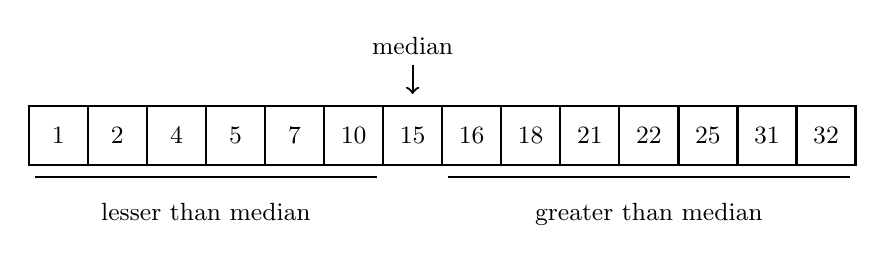
\begin{tikzpicture}[every node/.style={font=\small}, scale=0.75]

% --- Array values (10 elements) ---
\def\A{{1, 2, 4, 5, 7, 10, 15, 16, 18, 21, 22, 25, 31, 32}}
\def\MID{6} % Index of median (0-based): value = 23
% Draw array elements and indices
\foreach \i in {0,...,13} {
    \pgfmathsetmacro{\val}{\A[\i]}
    \draw[thick] (\i, 0) rectangle ++(1,1);
    \node at (\i+0.5, 0.5) {\val};
}

% Underline LEFT subarray (0..3)
\draw[thick] (0.1, -0.2) -- (6.0-0.1, -0.2);
% Label
\node[below=6pt] at (3, -0.2) {lesser than median};

% Underline RIGHT subarray (5..9)
\draw[thick] (7+0.1, -0.2) -- (13+1-0.1, -0.2);
% Label
\node[below=6pt] at (10.5, -0.2) {greater than median};

% Arrow for mid
\draw[<-, thick] (\MID+0.5, 1.2) -- +(0, 0.5) node[above] {median};

\end{tikzpicture}
\caption[Binary search]{Example of a sorted array containing 14 elements. }
\label{fig:binary-search-subarrays}
\end{figure}


The study of searching was initiated by D. Knuth in his seminal book \cite{Knuth1973} in which he discussed its various variants. However, the origins of the search problem reach the famous Rényi-Ulam game of twenty one questions in which a player is required to guess an unnamed object by asking yes-or-no questions\footnote{Note that in the twenty-one questions game one answer to a question may be a lie.}. Throughout the years, the searching and its variants have been continuously rediscovered under various definitions and names. This hints that the intuitions behind this problem resurface among multiple use cases and research domains. In fact, the search problem in its many variants is deeply connected with many other algorithmic notions including: parallelization of the Cholesky factorization, scheduling join operations in database queries, VLSI-layouts, learning theory, data clustering, graph cuts and parallel assembly of multi-part products. This work aims to serve as a survey of the results obtained for the problem and an experimental analysis of algorithms aimed at solving it.

The importance of searching is also due to its various practical applications. For example consider the following scenario: a complex procedure contains a hidden bug required to be fixed. The procedure is composed of multiple (often nested) blocks of code. In order to find this hidden bug the searcher can perform tests which allow him to check whether the given block of code contains the bug. After performing each such test they learn whether the bug is in or outside of the tested block. This process then continuous, until the bug is found. The problem is to find the best testing strategy for the tester in order to find the bug efficiently.

% A different scenario may occur in the medical diagnostics. The so called \textit{House M.D. Problem} is concerned with diagnosing a potentially lethal, hidden disease. In order to do so, House and his medical team perform series of tests on the patient. These tests (often avant-garde in their nature) may include blood tests, a family survey or even breaking into the patients house. After performing each such test the team learns some new information about the patient which allows them to iteratively narrow the size of the space of possible diagnoses. The outcome of such test may include for example: the sugar level in blood is low (or high), the patients mother died of a disease with similar symptoms, the patient consumes very large amount of tuna etc. As the condition of the patient is deteriorating rapidly, the team needs to determine the disease as quickly as possible. 


\chapter{Theorethical Analysis}

The following chapter is concerned with the presentation and theoretical analysis of the algorithms for the Search Problem. We partition the analysis into 5 main sections: Paths, Unitary costs in trees, Non-uniform costs in trees, Arbitrary graphs and Miscellaneous. The variants are grouped according to the similarity of structure, hardness and the techniques used to solve them. It should be noted that however this choice is arbitrary as sometimes distant versions of the problem remain connected and some techniques used to solve one version might be somewhat useful in the other.
%\section{Paths}
In general, all of the variants of the problem dealing with paths are known to be solvable in polynomial time. This is due to the fact that the number of subpaths of a path is of size $\binom{n}{2}=O\br{n^2}$. Such property allows us to construct efficient dynamic programming solutions, which when naively implemented, usually run in time $O\br{n^3}$. The key part of the analysis is often to show how to optimize such solution in order to reduce the factor of $O\br{n}$ thus obtaining $O\br{n^2}$ running time.
Let $V\br{P}=v_1,\dots,v_n$. In the following considerations by  $\OPT_{sum}\br{i,j}$ we will denote the cost of optimal decision tree for a subpath $v_i,..,v_j$ according to the average case cost and similarly by $\OPT_{max}\br{i,j}$ we will denote the cost of optimal decision tree for a subpath $v_i,..,v_j$ according to the worst case cost. Whenever clear from the context we will drop the subscript and simply write $\OPT\br{i,j}$. For both variants we have that $\OPT=\OPT\br{1,n}$. By a slight abuse of notation we will also use $\OPT\br{i,j}$ to denote the root query of the decision tree whose cost is equal to this value.
In this section we will be only concerned with the edge query model, as each of the constructed solutions can be easily altered to solve the vertex query version of the problem. The following paragraph introduces us with the general recurrence relationships exploited in the dynamic programming. 
\paragraph{A warm up: $O\br{n^3}$ algorithm for $P||E,c|| \COST_{max}$ and $P||E,c, w|| \sum C_i$}

First of all, following the definition of $\OPT\br{i,j}$ we get that $\OPT\br{i,i}=0$ for both worst and average case criteria.
Fix some $i<j$. The two next recurrence relationships stem from a fact that  there must exist some query among edges of $v_i,..v_j$ which is the root of the optimal decision tree. Define $D_{max}$ to be this decision tree (for the worst case cost) and $q_{max}=r\br{D_{max}}$ to be its root query. Let $P_1,P_2\in P-q_{max}$ and let $D_1, D_2\in D-q_{max}$ be the subtrees of $D_{max}$ being decision trees for $P_1$ and $P_2$ accordingly. Let $D_{max}'$ be the costiest of the two and $P_{max}'$ be the according path. We have that: $\OPT_{max}\br{i,j}=\COST_{max}\br{D_{max}}=c\br{q_{max}}+\COST_{max}\br{D_{max}'}$. 
By the optimality of $\OPT_{max}\br{i,j}$ we immediately obtain that $D_{max}'$ is the optimal decision tree for $P_{max}'$. This results in the following recurrence relationship:
$$
\OPT_{max}\br{i,j} = \min_{i\leq k<j}\brc{c\br{v_kv_{k+1}}+\max\brc{\OPT_{max}\br{i, k}, \OPT_{max}\br{k+1, j}}}
$$
Similarly, fix again $i<j$ and define $D_{sum}$ to be the optimal decision tree (for the average case cost) for $v_i,\dots,v_j$ and $q_{sum}=r\br{D_{sum}}$ to be its root query. Let $P_1,P_2\in P-q_{sum}$ and $D_1, D_2\in D-q_{sum}$ be the subtrees of $D_{sum}$ begin decision trees for $P_1$ and $P_2$ accordingly. Let $C\br{D_{sum}, x}$ denote the cost of finding $x\in\brc{v_i,\dots,v_j}$ using $D_{sum}$. Let $w\br{i,j}=\sum_{i\leq k\leq j}w\br{v_k}$. We have that:
$$
\OPT_{sum}\br{i,j}=\sum_{x\in v_i,\dots,v_j}w\br{x}\cdot \COST_{sum}\br{D_{sum}, x}=w\br{i,j}\cdot c\br{q_{sum}} + \COST_{sum}\br{D_1} + \COST_{sum}\br{D_2}
$$
By the optimality of $\OPT_{max}\br{i,j}$ we immediately obtain that $D_1$ is the optimal decision tree for $P_1$ and $D_2$ is the optimal decision tree for $P_2$. This results in the following recurrence relationship:
$$
\OPT_{sum}\br{i,j} = \min_{i\leq k<j}\brc{w\br{i,j}\cdot c\br{v_kv_{k+1}}+\OPT_{sum}\br{i, k}+ \OPT_{sum}\br{k+1, j}}
$$

Both recurrences can be solved using dynamic programming in time $O\br{n^3}$. To see this, recall that there are at most $\binom{n}{2}$ values for all possible choices of values of $i$ and $j$ and each of them requires checking at most $n-1$ choices for the root of the optimal decision tree.

Despite being polynomial, $O\br{n^3}$ is substantial amount of calculation for the practical purposes we are interested in. In subsequent considerations we show how, using clever tricks, lower down the running time of these dynamic programming algorithms in some special cases. 
\subsection{Average case, non-uniform weights}
\begin{theorem}
    There exists an $O\br{n^2}$ algorithm for $P||E, w|\sum C_i$
    \begin{proof}
        
The idea behind the speed-up described below is due to Knuth \cite{Knuth1973} and \cite{EffDPusingQI}. For every $i\leq k< j$ let $\OPT_k\br{i,j} = w\br{i,j} + \OPT\br{i, k} + \OPT\br{k, j}$ be the optimal cost of searching in $v_i,\dots,v_j$ assuming that the edge $v_kv_{k+1}$ is the root of the decision tree. We have that $\OPT\br{i,j}\leq \OPT_k\br{i,j}$. Additionally, define 
$K\br{i,j} = \max_{i\leq k< j}\brc{k|\OPT_k\br{i,j}=\OPT\br{i,j}}$ to be the largest index such that setting $v_kv_{k+1}$ as the root of the decision tree yields the optimal solution. 

Let $i \leq i' \leq j \leq j'$.
Observe that the weight function fulfills the following inequalities:
\begin{enumerate}
\item Monotocity: $w\br{i',j}\leq w\br{i,j'}$
\item The quadrangle inequality (QI):
$
w\br{i,j} + w\br{i',j'}\leq 
w\br{i',j} + w\br{i,j'}
$
\end{enumerate}
Using the above fact we will firstly show the following:
\begin{lemma}
   The $\OPT$ function satisfies the quadrangle inequality
   \begin{proof}
       Let $i \leq i' \leq j \leq j'$. The proof is by induction on $l=j'-i$. Assume by induction that:
       $$\OPT\br{i,j} + \OPT\br{i',j'}\leq 
\OPT\br{i',j} + \OPT\br{i,j'}$$
Whenever $i=i'$ or $j=j'$ the claim follows trivially and therefore is true for $j\leq 1$ so assume otherwise. There are two cases:
\begin{enumerate}
   \item $i'=j$.
   Let $k=K\br{i,j'}$. In this case the inequality reduces to $\OPT\br{i,j} + \OPT\br{j,j'}\leq \OPT\br{i,j'}$. There are two subcases:
   \begin{enumerate}
       \item $k\leq j$.
       We have that:
       \begin{align*}
       \OPT\br{i, j} + \OPT\br{j, j'} &\leq \OPT_k\br{i, j} + \OPT\br{j, j'} 
       \\ 
       &= 
       w\br{i, j} + \OPT\br{i, k} + \OPT\br{k+1, j} + \OPT\br{j, j'}
       \\ 
       &\leq
       w\br{i, j'} + \OPT\br{i, k} + \OPT\br{k+1, j'} 
       \\
       &=
       \OPT_k\br{i, j'} \\
       &= \OPT\br{i, j'}
       \end{align*}
       Where the first inequality and the first equality are due to the definition of $\OPT_k$, the second inequality is due to monotonicity of $w$ and the induction hypothesis and the last two equalities are again due to the definition of $\OPT_k$.
        \item The case when $k\geq j$ is symmetrical.
   \end{enumerate}
    \item $i' < j$.
    Let $y=K\br{i',j}$ and $z=K\br{i,j'}$. There are again two symmetric cases:
    \begin{enumerate}
        \item $z\leq y$. We have that:
        \begin{align*}
        &\OPT\br{i, j} + \OPT\br{i', j'} \\
        &\leq \OPT_z\br{i, j} + \OPT_y\br{i', j'} \\
        &=w\br{i, j} + w\br{i', j'} + \OPT\br{i, z} + \OPT_z\br{z+1, j} + \OPT_y\br{i', y} + \OPT_y\br{y+1, j'} \\
        &\leq w\br{i', j} + w\br{i, j'} + \OPT\br{i, z} + \OPT_y\br{i', y} + \OPT_z\br{y+1, j} + \OPT_y\br{z+1, j'}\\
        &= \OPT_y\br{i', j} + \OPT_z\br{i, j'} \\
        &= \OPT\br{i', j} + \OPT\br{i, j'}
        \end{align*}
        Where the first inequality and the first equality are due to the definition of $\OPT_k$, the second inequality is due to QI of $w$ and the induction hypothesis at $z\leq y<j < j'$ and the last two equalities are again due to the definition of $\OPT_k$.
        \item Also this time the other case when $k\geq j$ is symmetrical.
    \end{enumerate}
\end{enumerate} 
   \end{proof}
\end{lemma} 
Having the above lemma we will now prove the following:
\begin{lemma}
   $K\br{i,j-1}\leq K\br{i,j}\leq K\br{i +1,j}$
   \begin{proof}
   To prove the first inequality $K\br{i,j-1}\leq K\br{i,j}$ we will show that for $i\leq k \leq k' < j$ we have that: $\OPT_{k'}\br{i, j - 1} \leq \OPT_{k}\br{i, j - 1}$ implies that $\OPT_{k'}\br{i, j} \leq \OPT_{k}\br{i, j}$. This condition suffices as whenever $k'=K\br{i, j - 1}$ this means that either $k'=k$ or $k\neq K\br{i, j}$ as choosing $v_{k'}v_{k'+1}$ as the root of the decision tree provides a solution which cannot be worse\footnote{Note that by the definition we require $K\br{i, j}$ to be maximal.}. By using QI at $k\leq k'\leq j -1< j$ we have:
   $$
   \OPT\br{k, j-1} + \OPT\br{k', j}\leq \OPT\br{k', j-1} + \OPT\br{k, j}
   $$
   By adding $w\br{i,j-1}+w\br{i,j}+\OPT\br{i, k}+\OPT\br{i, k'}$ to both sides we obtain:
   $$
   \OPT_k\br{i, j-1} + \OPT_{k'}\br{i, j-1} \leq \OPT_{k'}\br{i, j-1} + \OPT_{k}\br{i, j-1}
   $$
   Which implies the claim. 
   The second inequality $K\br{i,j}\leq K\br{i +1,j}$ follows similarly from the QI at $i < i+1 \leq k \leq k' $.
   \end{proof}
\end{lemma}
 
The above lemma allows us to the amount of computation required. The idea is as follows: Before calculating $\OPT\br{i,j}$ we firstly calculate the values of $\OPT\br{i -1,j}$ and $\OPT\br{i,j + 1}$. In doing so we also calculate the indices $K\br{i,j-1}$ and $K\br{i +1,j}$ required to narrow the space of possible choices for value of $K\br{i,j}$. We obtain the following recurrence relationship:
$$
\OPT_{sum}\br{i,j} = \min_{K\br{i,j-1}\leq k\leq K\br{i +1,j}}\brc{w\br{i,j}+\OPT_{sum}\br{i, k}+ \OPT_{sum}\br{k+1, j}}
$$
It remains to show that the running time can be bounded by $O\br{n^2}$. The amount of computation steps required by the algorithm is equal to:
\begin{align*}
\sum_{i=1}^n\sum_{j=i+1}^n\br{K\br{i + 1, j} - K\br{i,j - 1}} &= \sum_{i=1}^n\sum_{j=i}^n\br{K\br{i + 1,j+1} - K\br{i,j}}
\\
&=\sum_{i=1}^n\br{K\br{i + 1,n}-K\br{1,i}} = O\br{n^2}
\end{align*}
Where the second equality is due to the fact that all of the terms except $K\br{i + 1,n}$ and $K\br{1,i}$ cancel, and the last equality is trivially due to the fact that $K\br{i + 1,n} < n$. This proves the claim.
    \end{proof}
\end{theorem}
\subsection{Non-uniform costs, worst case}
Lorem ipsum dolor sit amet, consectetur adipiscing elit, sed do eiusmod tempor incididunt ut labore et dolore magna aliqua. Ut enim ad minim veniam, quis nostrud exercitation ullamco laboris nisi ut aliquip ex ea commodo consequat. Duis aute irure dolor in reprehenderit in voluptate velit esse cillum dolore eu fugiat nulla pariatur. Excepteur sint occaecat cupidatat non proident, sunt in culpa qui officia deserunt mollit anim id est laborum.
\subsection{Non-uniform costs, Average case, uniform weights}
Lorem ipsum dolor sit amet, consectetur adipiscing elit, sed do eiusmod tempor incididunt ut labore et dolore magna aliqua. Ut enim ad minim veniam, quis nostrud exercitation ullamco laboris nisi ut aliquip ex ea commodo consequat. Duis aute irure dolor in reprehenderit in voluptate velit esse cillum dolore eu fugiat nulla pariatur. Excepteur sint occaecat cupidatat non proident, sunt in culpa qui officia deserunt mollit anim id est laborum.

\newpage
\SetKwFunction{FRankingBasedDT}{RankingBasedDT}
\section{Trees, Worst Case, Uniform Costs}


% \subsubsection{Vertex ranking}\label{vertexRanking}
The \textit{vertex ranking} of $T$ is a labeling of vertices $l:V\to \brc{1,2,\dots,\cl{\log n}+1}$, which satisfies the following condition: for each pair of vertices $u,v\in V\br{T}$, whenever $l\br{u}=l\br{v}$, there exists $z\in \mathcal{P}_T\br{u,v}$ for which $l\br{z}>l\br{v}$. Such a labeling always exists and can be computed in linear time by means of dynamic programming \cite{Schaffer1989OptNodeRankOfTsInLinTime, OnakParys2006GenOfBSSInTsAndFLikePosets, Mozes_Onak2008FindOptTSStartInLinTime}. For a visual example, see Figure \ref{vertex_ranking_figure}

\begin{figure}[htbp]
    \centering
    \begin{minipage}{0.26\textwidth}
        \centering
        \tikz [tree layout, grow=-65,
               sibling distance=7mm, level distance=11mm,]
          \graph {
    ""[as=$a$] -- {
        ""[as=$b$] -- ""[as=$c$] -- {
            ""[as=$d$] -- ""[as=$e$],
            ""[as=$f$] -- { ""[as=$g$], ""[as=$h$], ""[as=$i$] }
        },
        ""[as=$j$] -- ""[as=$k$] -- { ""[as=$l$], ""[as=$m$] }
    }
};
    \caption[Sample tree with uniform costs]{}
    \label{vr_tree}
    \end{minipage}
    \begin{minipage}{0.26\textwidth}
        \centering
        \tikz [tree layout, grow=-65,
               sibling distance=7mm, level distance=11mm,]
          \graph {
    ""[as=$4$] -- {
        ""[as=$1$] -- ""[as=$3$] -- {
            ""[as=$2$] -- ""[as=$1$],
            ""[as=$2$] -- { ""[as=$1$], ""[as=$1$], ""[as=$1$] }
        },
        ""[as=$1$] -- ""[as=$2$] -- { ""[as=$1$], ""[as=$1$] }
    }
};
    \caption[Sample tree with uniform costs]{}
    \label{vr_ranking}
    \end{minipage}
    \begin{minipage}{0.45\textwidth}
        \centering
        \tikz [tree layout, grow=-90,
               sibling distance=8mm, level distance=15.5mm,]
            \graph {
              ""[as=$a$] -> {
                ""[as=$c$] -> {""[as=$b$], ""[as=$d$] -> {""[as=$e$]}, ""[as=$f$] -> {""[as=$g$], ""[as=$h$], ""[as=$i$]}}, ""[as=$k$]->{""[as=$j$], ""[as=$l$], ""[as=$m$]}
              }
            };
        \caption[Edge decision tree for a tree]{}
        \label{vr_dt}
    \end{minipage}
        \caption[Tree and decision trees for it]{Sample input tree $T$ (Figure \ref{vr_tree}), vertex ranking labeling $l$ of $T$ (Figure \ref{vr_ranking}) and a decision tree $D$ for $T$ built using $l$ (Figure \ref{vr_dt}).}
        \label{vertex_ranking_figure}
\end{figure}

Having a vertex ranking of $T$, one can easily obtain a decision tree for $T$ using the following procedure:
\begin{enumerate}
    \item Let $z\in V\br{T}$ be the unique vertex, such that for every $v\in V\br{T}$, $l\br{z}\geq l\br{v}$.
    \item Schedule a query to $z$ as the root of the decision tree $D$ for $T$.
    \item For each $T'\in T-z$, build a decision tree $D_{T'}$ recursively and hang it below the query to $z$ in $D$.
\end{enumerate} 

When the input tree has uniform costs and the ranking uses the minimal number of labels, the decision tree built in this way is optimal and never uses more than $\fl{\log n} + 1$ queries \cite{OnakParys2006GenOfBSSInTsAndFLikePosets}. Let \FRankingBasedDT be the name of the latter procedure. We have the following corollary:
  
\begin{corollary}\label{vertexRankingCorollary}
    There exists an $O\br{n}$ time procedure \FRankingBasedDT that finds the optimal decision tree for the Tree Search Problem when all costs are uniform. Moreover, the depth of such a decision tree, i.e., the worst-case number of queries, is at most $\fl{\log n} + 1$.
\end{corollary}

We assume that the input tree is rooted at an atribtarry vertex.
Below we show how to calculate the optimal vertex ranking of a given tree $T$. For any vertex $v\in V\br{T}$, and any coloring $l$ we define the \textit{visibility sequence} $S\br{v}$ as following: let $l\in \mathbb{N}$. If there exists a vertex $u\in V\br{T}$, such that for every $z\in\mathcal{P}_T\br{u,v}$, $l< l\br{z}$, then $l\in S\br{v}$. We also demand that $S\br{v}$ is sorted decreasingly. If for given label $l$, $l\in S\br{v}$, we say that such label is \texit{visible} from $v$. In order to find the coloring using the minimal amount of colors, we will make use of the standard lexicographic order on visibility sequences. Notice, that for any vertex $v\in V\br{T}$, we have that $\max_{u\in V\br{T}}\brc{l\br{u}}\in S\br{v}$. Therefore, a labeling with the lexycogrophically lowest $S\br{r\br{T}}$ is also an optimal. We focus ourselves on finding such labeling. We devise the following dynamic programming procedure which calculates a labeling of $T$ with a minimal visibility sequence of $r\br{T}$.

\SetKwFunction{FCalculateRanking}{CalculateRanking}
\begin{algorithm}
\caption{The \FCalculateRanking procedure.}\label{calculateRanking}
\SetKwProg{Fn}{Procedure}{:}{}
\Fn{$\FCalculateRanking\br{T}$}{
    \For{$1\leq j\leq \deg_{r\br{T}}^+$}{   
        $S\br{c_j}\gets \FCalculateRanking\br{T_{c_j}}$.
    }

    $m\gets$ maximal value belonging to at least two distinct $S\br{c_j}$.

    $S\br{v}\gets \bigcup_{j=1}^{\deg_{r\br{T}}^+} S\br{c_j}$.

    $l\br{r\br{T}}\gets \argmin_{m < k \leq \log n + 1, k \notin S\br{v}}\brc{k}$.

    Append $l\br{v}$ to $S\br{v}$.

    Remove any $l < l\br{v}$ from $S\br{v}$.

    \Return $S\br{v}$.
}
\end{algorithm}

The following theorem is by \cite{OnakParys2006GenOfBSSInTsAndFLikePosets}:
\begin{theorem}
    Let $T$ be a tree. The Algorithm \ref{calculateRanking} can be implemented in $O\br{n}$ time and returns a correct ranking labeling such that $S\br{r\br{T}}$ islexycogrophically optimal.
\end{theorem}


\newpage
\section{Average case, non-uniform weights}
The problem of average case searching is also solvable in polynomial time assuming all of the weight are uniform. However the procedure is the same as for the weighted case and only the running time differ. Hence we combine these results in one section. Note that it is yet unknown whether the same holds for the weighted version of the problem and the fastest known algorithm runs in pseudopolynomial time. Using this one may also obtain a FPTAS using a standard rounding trick. Before that, however we show that a simple greedy heuristics achieves a 2-approximation for $T|V,w|\sum C_j$.
\subsection{Greedy achieves 2-approximation for $T|V,w|\sum C_j$}
The weight centroid is a vertex $c\in T$ such that for every $H\in T-c$ we have that $w\br{h}\leq \frac{w\br{T}}{2}$. The existence of the (unweighted) centroid has been known since 19th century \cite{Jordan1869}. The proof of the existence of the weight centroid i straightforward and can be summarized as follows: pick any vertex $v\in T$ and if its not a weight centroid move to the neighbor $v'$ of $v$ such that the $H\in T-v$ such that $v'\in H$ has weight $w\br{H}>\frac{w\br{T}}{2}$. It is easily observable that the algorithm always succeeds and visits each vertex at most once. The greedy algorithm is as follows: pick the centroid $c$ of $T$ as the root of the decision tree for $T$ and proceed recursively in $T-c$. The following analysis of greedy is due to \cite{Fast_app_centroid_trees}.

\begin{theorem}
    Let $D_c$ be the greedy decision tree. Then $\COST_{D_c}\br{T}\leq 2\OPT\br{T}-w\br{T}$.
    \begin{proof}
        We start with the following lemma:
        \begin{lemma}\label{lemma:avg_lb_centroid}
            Let $D$ be any decision tree for $T$ and let $c$ be the centroid of $T$. Then:
            $$
            \OPT\br{T}\geq \frac{w\br{T}}{2}+\frac{w\br{c}}{2}+\sum_{H\in T-c}\OPT\br{H}
            $$
            \begin{proof}
                Let $r=r\br{D}$. There are two cases:
                \begin{enumerate}
                    \item $r=c$. In such case the cost of the solution is trivially lower bounded by:
                    $$
                    \COST_{D}\br{T}\geq w\br{T}+\sum_{H\in T-r}\OPT\br{H}\geq \frac{w\br{T}}{2}+\frac{w\br{c}}{2}+\sum_{H\in T-c}\OPT\br{H}
                    $$
                    \item $r\neq c$. In such case denote by $H_r$ the connected component of $T-c$ such that $r\in H_r$. We have that the contribution of each $v\in H_r$ is at least $\spr{Q_{D|H_r}\br{v}}$ so the overall contribution of vertices in $H_r$ is at least $\COST_{D|H_r}\br{H_r}$. For every $H\in T-c$ such that $H\neq H_r$ and $v\in H$ we have that $\brc{r}\cup Q_{D|H}\br{v}\subseteq Q_{D}\br{v}$ so we have that the contribution of vertices in $H$ is at least $w\br{H}+\COST_{D|H}\br{H}$. Additionally the contribution of $c$ is at least $w\br{c}$ since query to $r$ precedes the query to $c$. We have that:
                    \begin{align*}
                        \COST_D\br{T}&\geq 2w\br{c}+\COST_{D|H_r}\br{H_r}+\sum_{H\in T-c, H\neq H_r}\br{w\br{H}+w\br{c}+\COST_{D|H}\br{H}}\\
                        &\geq w\br{T}-w\br{H_r}+\sum_{H\in T-c}\OPT_{D|H}\br{H}\\
                        &\geq \frac{w\br{T}}{2}+w\br{c}+\sum_{H\in T-c}\OPT_{D|H}\br{H}
                    \end{align*}
                    where in the last inequality we used the fact that $c$ is a centroid of $T$.
                \end{enumerate}
            \end{proof}
        \end{lemma}
        The proof is by induction on the size of $T$. When $n\br{T}=1$ we have that $\COST_{D_c}\br{T}=w\br{T}=2\OPT\br{T}-w\br{T}$. Assume therefore that $n\br{T}>1$ and let $c$ be the centroid of $T$. We have that:
        \begin{align*}
            \COST_{D_c}\br{T} &= w\br{T}+\sum_{H\in T-c}\COST_{D_c|H}\br{H}\\
            &\leq w\br{T}+\sum_{H\in T-c}\br{2\cdot\OPT\br{H}-w\br{H}}\\
            &= w\br{c}+\sum_{H\in T-c}2\cdot\OPT\br{H}\\\
            &\leq 2\OPT\br{T}-w\br{T}
        \end{align*}
        where the first inequality is by the induction hypothesis and the second inequality is by the Lemma \ref{lemma:avg_lb_centroid}.
    \end{proof}
\end{theorem}
\begin{theorem}
    The greedy decision tree can be found in $O\br{n\log n}$ running time.
    \begin{proof}
        We use the data structure called \textit{top trees}. The top trees are used to maintain dynamic forests under
insertion and deletion of edges. The following theorem is due to \cite{toptrees}:
    \begin{theorem}
        We can maintain a forest with positive vertex weights on n vertices
under the following operations:
\begin{enumerate}
    \item Add an edge between two given vertices $u$, $v$ that are not in the same connected component.
    \item Remove an existing edge.
    \item Change the weight of a vertex.
    \item Retrieve a pointer to the tree containing a given vertex.
    \item Find the centroid of a given tree in the forest.
\end{enumerate}
Each operation requires $O\br{\log n}$ time. A forest without edges and with n arbitrarily weighted vertices can be
initialized in $O\br{n}$ time.
    \end{theorem}
        We begin with building the top tree out of $T$. We begin with empty top tree and add each edge one by one. Then we find the centroid of $T$ and remove each edge incident to it. Then we recurse on this new created tree (excluding the subtree consisting of $c$). Since the algorithm finds each vertex once and removes each edge once the total running time is of order $O\br{n\log n}$.
    \end{proof}
\end{theorem}

\subsection{PTAS for $T|V,w|\sum C_j$}
\begin{theorem}
    Fix $\epsilon>1$. There exists an $\br{1+\epsilon}$-approximation algorithm for $T||V, w||\sum C_i$ running in $O\br{n^{\br{2/\epsilon+3}}\log n/\epsilon}$ time.
    \begin{proof}

To design our PTAS we will make use of the following lemma combined with a non trivial dynamic programming procedure due to \cite{Cicalese2014ImprovedApproxAvgTs,Angelidakis2018ShortestPQ, Berendsohn2024}. Note that, this is not the only way to obtain PTAS, see \cite{SplayTonT}.
\begin{lemma}\label{ptas_lemma}
Fix $\epsilon>1$. For every tree $T$, there exists a decision tree $D$, such that:
\begin{enumerate}
    \item $\COST_{avg,D}\br{T,w}\leq \br{1+\epsilon}\cdot\OPT_{avg}\br{T,w}$,
    \item $\COST_{max,D}\br{T,w}\leq \br{1+\frac{1}{\epsilon}}\cdot\br{\fl{\log n}+1}$
\end{enumerate} 
\begin{proof}
Let $D^*$ be any optimal startegy for $T$. If  $\COST_{max,D}\br{T,w}\leq \fl{\log n}+1$, then the claim follows. Assume contrary. In such case let $T'$ be any non empty subtree of $T$ occuring as the candidate subtree after first ${\fl{\log n}+1}/{\epsilon}$ queries of some branch of the strategy. We build $D$ by altering $D^*$ from now on. At each next level of the decision tree a centroid of a current candidate subtree is scheduled to be queried. In such case each vertex belonging to $T'$ gains additional query time equal to at most $\log \fl{\log n\br{T'}}+1\leq \fl{\log n}+1$ and the depth of $D$ is bounded by $\COST_{max,D}\br{T,w}\leq \br{1+\frac{1}{\epsilon}}\cdot\br{\fl{\log n}+1}$. Additionally, the cost of $D$ is at most:
\begin{align*}
    \COST_{avg,D}\br{T,w}&\leq 
\sum_{v \in V\br{T}}w\br{v}\br{\epsilon\cdot \spr{Q_{D^*}\br{T,v}}+\spr{Q_{D^*}\br{T,v}}}
\\&\leq
\br{1+\epsilon}\cdot \COST_{avg,D^*}\br{T,w}=
\br{1+\epsilon}\cdot\OPT_{avg}\br{T,w}
\end{align*}

\end{proof}
\end{lemma}

We assume that the input tree $T$ is rooted at an arbitrary vertex. If the response to a query contains $r\br{T}$ we say that such response is an \textit{up} response and we say that it is an \textit{down} response otherwise. Let $D$ be a decision tree for $T$. We say that a child of $q\in V\br{D}$ is a \textit{left} child if it is associated with an up response to query at $q$. We say that, it is a \textit{right} response otherwise. Note that any query in $D$ may have at most one left child.

To devise our dynamic program, we will need to use the following generalization of decision trees. An \textit{extended decision tree} $D=V\br{V\br{D}, E\br{D}}$ for the tree $T$ is defined analogously as ordinary decision tree, however we allow $V\br{D}=V\cup U \cup B$, where $V\subseteq V\br{T}$, $U$ is a set of nodes in $V\br{D}$ labeled as \textit{unassigned} and $B$ is a set of nodes in $V\br{D}$ label as \textit{blocked}. We also require if $q\inV\br{D}\in U\cup B$, then $q$ has no right children. The cost of such decision tree is defined the same as the cost of an ordinary decision tree. Note that, any decision tree is also an extended decision tree, and we can easily transform any extended decision tree to obtain an ordinary decision tree. To do so, simply delete every query $q\in U\cup B$. If $q\neq r\br{D}$ and $q$ has a left child, then: If $q$ was a left child of $p\br{q}$, hang the left child of $q$ as a left child of $p\br{q}$. Else if $q$ was a right child of $p\br{q}$, hang the left child of $q$ as a right child of $p\br{q}$.

We will also define a \text{timeline} $P$ to be an extended decision tree consisting of sequence of queries $\angl{p_1,\dots,p_k}$, such that every query of $P$ is either blocked or unassigned. We will build our decision trees around timelines. Let $D$ be any extedned decision tree. Define the \textit{left path} $P_D=\angl{q_1,\dots,q_h}$ of $D$ as the sequence of queries in $D$, obtained by traversing $D$ starting from $r\br{D}$, and stepping to the left child until there is none. We will say that $D$ with a left path $P_D=\angl{p_1,\dots,p_k}$ is \textit{compatible} with a timeline $P=\angl{q_1,\dots,q_h}$, such that $k\leq k$ if for every integer $1\leq l \leq h$, if $q_k\in B$, then $p_k\in B$. 

We will now introduce the subproblems which our dynamic programming solves. A problem $\OPT\br{T_{v,i}, P}$ consist of finding an optimal extended decision tree for the tree $T_{v,i}$, which is compatible with $P$. Additionally, a global parameter $h$ is given which bounds the maximum height of the solution found by the algorithm and in consequence, the length of $P$. The algorithm will compute the solutions to subproblems in an bottom-up and left to right manner. If at any point there is no way to create an extended decision tree with given parameters we simply declare such instance \textit{unfeasible}. The choice of the constant $h$ will ensure existence of at least one such solution. We will now show how to compute $\OPT\br{T_{v,i}, P}$ efficiently. There are 3 cases:

\input{pseudocodes/dp_timelines.tex}

    \begin{enumerate}
        \item \textbf{$T_{v,0}$}
        
            In this case we greedily pick the smallest index $1 \leq k \leq \spr{P}$ such that $p_k$ is unassigned. If there is no such index, we declare the subproblem unfeasible. In other case the solution obtained by taking timeline $P$ and setting $p_k=v$. The cost of such solution is $w(v)\cdot k$.
        \item \textbf{$T_{v,1}$}
        
        Let $u$ be the unique child of $v$ in $T_{v,1}$. We assume that we have already solved all the sub-problems of $T_u$.
            In this case we iterate through all possible choices of $1\leq k \leq h$ such that $p_k$ is unassigned. If there are no such we declare the subproblem unfeasible. If otherwise for each such $k$ we create an auxiliary timeline $P_k'=
            \angl{p_1',\dots,p_h'}$ such that $p_l'=p_l$ for $l < k$, $p_k'$ is blocked and $p_l'$ is unassigned for $l>k$. We consider an optimal extended decision tree $D'_k$ for an instance $\mathcal{P}\br{T_{u}, P_k'}$. In order to create a new decision tree $D_k$ for each choice of $k$ we proceed as follows: Let $q'_k$ be the $k$-th vertex of the left path of $D'_k$. We set $q'_k=v$ Then, we take the left child of $q'_k$ in $D'$ and we rehang it as the right child of $q'_k$. Additionally we fill the left path of $D'$ with blocked and unassigned vertices in order to make it again compatible with $P$.
            The cost of each such extedned decision tree is $\OPT\br{T_{u}, P_k'}+w(v)\cdot k$. We then choose an optimal extended decision tree $D$, which minimizes the cost.
        \item \textbf{$T_{v,i}$ for $i>1$}
        
        We assume that we have already solved all the subproblems of $T_{v,i-1}$ and $T_{c_i}$. Let $I$ be a set of indices of unassigned nodes of $P$, i.e. $I=\brc{l | p_l \text{ is unassigned}}$. Consider any bipartition $\br{I_1, I_2}$ of $I$. We create a timeline $P_1=\angl{p_{1,1},\dots,p_{1,h}}$ from timeline $P$ by blocking all of the nodes whose indices do not belong to $I_1$. We now consider an extended decision tree $D_1$ for $\mathcal{P}\br{T_{v,i-1}, P_1}$ with a left path $\angl{q_{1,1},\dots,q_{1,d_1}}$. Let $k$ be the index of query to $v$, such that $q_{1,k}=v$. We construct $P_2=\angl{p_{2,1},\dots, p_{2,h}}$ as follows: for any $1\leq l\leq h$, we set $p_{2,l}$ to be unassigned if $l\in I_k^2$ or $l < k$ and we set $p_{2,l}$ to be blocked otherwise. Let $D_2$ be an optimal extended decision tree for $\mathcal{P}\br{T_{c_i}, P_2}$ and let $\angl{q_{2,1},\dots,q_{2,d_2}}$ be its left path. We proceed as follows. Firstly, we rehang the left child of $q_{2,k}$ in $D_2$ as its unique right child (by construction $q_{2,k}$ is blocked in $D_2$). Then we take the "union" of $D_1$ and $D_2$ by aligning their left paths. Since the unassigned nodes above the $k$-th node of left paths of $D_1$ and $D_2$ have no conflicts and $D_2$ has no vertices in its left path beyond $q_{2,k}$, by construction we obtain a valid extended decision tree $D$. The cost of such solution is $\OPT\br{T_{v,i-1}, P_1}+\OPT\br{T_{c_i}, P_2}$. We then choose an optimal extended decision tree $D$, which minimizes the cost.
    \end{enumerate}
    
\input{figures/dp_timelines.tex}
    Let $P=\angl{p_1,\dots,p_h}$, such that for every integer $1\leq k \leq h$, $p_k\in U$. Let $h=\br{1+\frac{1}{\epsilon}}\cdot\br{\fl{\log n}+1}$. Since, any extended decision tree of depth at most $h$ is compatible with $P$ by Lemma \ref{ptas_lemma} we have that for $D$ calculated for $\OPT\br{T, P}$,
    $\COST_{D}\br{T,w}\leq \br{1+\epsilon}\cdot\OPT\br{T,w}$.

    There are at most $O\br{n}$ subtrees $T_{v,i}$, $2^h$ different timelines and each subproblem requires $O\br{h+2^hh}=O\br{2^hh}$ amount of computation, since there are at most $2^h$ bipartitions of unassigned vertices of any timeline and aligning two decision trees requires $O\br{h}$ time. Therefore the running time of the procedure is bounded by $O\br{n\cdot 2^{2h}h}=O\br{n^{\br{2/\epsilon+3}}\log n/\epsilon}$ as required.
    
\end{proof}
\end{theorem}

\begin{algorithm}
\caption{The FPTAS for $T||V,w,||\sum C_i$}\label{fptas}
\SetKwFunction{FFPTAS}{FPTAS}
\SetKwProg{Fn}{Procedure}{:}{}
\Fn{$\FFPTAS\br{T, w, \epsilon}$}{
$K\gets\frac{\epsilon\cdot w\br{T}}{n^2}$.

\ForEach{ $v\in V\br{T}$}
{$w'\br{v} \gets \cl{\frac{w\br{v}}{K}}$.}

$h\gets \cl{\log_{3/2}w'\br{T}}$.

$P\gets\angl{p_1,\dots,p_h}$, such that for every $1\leq k\leq h$, $p_h\gets \textit{unassigned}$.

$D'\gets\FDPTimelines\br{T, w', P, h}$.

\Return $D'$.
}
\end{algorithm}
\SetKwFunction{FQPTAS}{QPTAS}
\newpage
\section{Trees, worst case, non-uniform costs}
% In this section we will be only concerned with the vertex-query variant of the problem. This is due to the fact that the edge variant is easily reducible to the vertex variant of the problem and this reduction preserves the approximation ratio (note that this reduces the problem to the version in which the last query may be omitted but all of the algorithms can be easily altered to consider this assumption). This is done by subdividing each edge $e$ with a new vertex $v_e$ of cost $c\br{v_e}=c\br{e}$. If we consider the average case criterion then we additionally set $w\br{v_e}=0$. It is immediate that the optimal decision tree for the this vertex query model instance can be used to obtain a decision tree for the original instance. To do so, simply replace each query to vertex $v_e$ with the query corresponding to $e$. 

The problem for non-uniform is NP-hard even when restricted to spiders of diameter $6$ and binary trees.
A simple greedy heuristics which always queries the middle vertex of the graph achieves a $O\br{\log n}$-approximation \cite{Dereniowski2009ERankOfWTs}. However one can obtain better results. 
We begin with the following simple lemma, which will become useful in few arguments:
\begin{lemma}\label{lemma:subtreeCost}
    Let $T'$ be a connected subtree of $T$. Then, $\OPT\br{T'}\leq\OPT\br{T}$.
\end{lemma}


\subsection{A warm up: $O\br{\log n/\log\log n}$-approximation algorithm  for $T||V,c||C_{max}$}
This first algorithm is an adapted and simplified version of the algorithm due to \cite{Cicalese2016OnTSPwNonUniCost} for the edge query model.
\begin{theorem}
    There exists a polynomial time, $O\br{\log n/\log\log n}$-approximation algorithm for the $T||V,c||C_{max}$ problem .
    \begin{proof}
        
To construct a decision tree we will use the following exact procedure:
\begin{lemma}
    There exists a $O\br{2^nn}$ algorithm for $T||V,c||C_{max}$
    \begin{proof}
        The algorithm is a general version of the dynamic programming procedure for paths. We have that:
        $$
        \OPT_{max}\br{T} = \min_{v\in V\br{T}}\brc{c\br{v}+\max_{H\in T-v}\brc{\OPT_{max}\br{H}}}
        $$
        There are there are at most $O\br{2^n}$ different subtrees of $T$ to be checked. Additionally, and for each $v\in V\br{T}$ there are at most $\deg_T\br{v}$ possible responses to check in the inner $\max$ function. Therefore for each subproblem there are at most
        $
        \sum_{v\in V\br{T}}\deg_T\br{v} = 2m = 2n-2
        $
        comparison operations to be performed. As at each level of the recursion the algorithm considers all possible choices of the next queried vertex $v$ it returns the optimal decision tree for $T$ and the claim follows.
    \end{proof}
\end{lemma}
\begin{observation}\label{neighborsPathObservation}
    Let $D$ be a partial decision tree for tree $T$. Let $T'$ be a subtree of $T$. Let $Q$ be a set of all queries to vertices from $N_{T}\br{V\br{T'}}$ in $D$ such that every for every $q\in Q$: $q$ is queried before every vertex in $T'$. Then $D\angl{Q}$ is a path. 
    \begin{proof}
        Let $x\in N_{T}\br{V\br{T'}}$. In such case, for every vertex $v\in V\br{T-V\br{T'}-N_{T}\br{V\br{T'}}}$ the answer to a query to $v$ is always towards the same $u\in N_{T}\br{v}$, so until a vertex from $T'$ is queried, no query $q$ can partition vertices from $N_{T}\br{V\br{T'}}$ into disjoint subtrees of candidate vertices except when $q\in N_{T}\br{V\br{T'}}$. After a query to $q$, the only different response is when $x=q$, in which case no further queries are needed, so queries in $Q$ must belong to a path in $D$.
    \end{proof}
\end{observation}



Let $k=2^{\fl{\log\log n}+2}$.
The basic idea is as follows. The algorithm is recursive. Let $\mathcal{T}$ be the tree currently processed by the algorithm. If $n\br{T}\leq k$ then we use the exponential time algorithm to find the optimal solution in time $2^kk=\text{poly}\br{n}$.

If otherwise, to build a solution (see Algorithm \ref{cicaleseInspired}) we will firstly define a set $\mathcal{X}\subseteq V\br{\mathcal{T}}$ which will be of size at most $k$. We build $\mathcal{X}$ iteratively. Starting with an empty set we pick the centroid $x_1$ of $T$ which we add to $\mathcal{X}$. Then we take the forest $F=T-x$, find the largest $H\in F$, pick its centroid $x_2$ and append it to $\mathcal{X}$. We continue this in $F-H + \br{H-x_2}$ until $\spr{\mathcal{X}}=k$.
\begin{lemma}\label{lemma:componentSize}
    For every $H\in \mathcal{T}-\mathcal{X}$ we have that $n\br{H}\leq n\br{\mathcal{T}}/\log\br{n}$.
    \begin{proof}
        We prove by induction on $t$ that deleting first $2^t$ centroids from $T$ each connected components $H_t$ has size at most $n\br{H_t}\leq n\br{\mathcal{T}}/2^{t-1}$. For the case when $t=0$ we have that after 1 iteration every $H_1$ has size at most $n\br{T}/2\leq 2\br{n}$ so the base of induction is complete.

        Fix $t>0$ and by assume by the induction hypothesis that after $2^{t-1}$ iterations all
    \end{proof}
\end{lemma}

We also define set $\mathcal{Y}\subseteq V\br{\mathcal{T}}$ which consists of vertices in $\mathcal{X}$ and all vertices in $v\in \mathcal{T}\angl{X}$ such that $\deg_{T\angl{\mathcal{X}}}\br{v}\geq 3$.
Furthermore, we define set $\mathcal{Z}\subseteq V\br{\mathcal{T}}$ as a set consisting of vertices in $\mathcal{Y}$ and for every $u,v\in \mathcal{Y}$ such that $\mathcal{P}_{\mathcal{T}}\br{u, v}\neq\emptyset$ and $\mathcal{P}_{\mathcal{T}}\br{u, v}\cap \mathcal{Y}=\emptyset$ we add to $\mathcal{Z}$ the vertex $\argmin_{z\in \mathcal{P}_{\mathcal{T}}\br{u, v}}\brc{c\br{z}}$ (for example see Figure \ref{exampleTreeWithSetZ}). We then create an auxiliary tree $\mathcal{T}_{\mathcal{Z}}=\br{\mathcal{Z},\brc{uv|\mathcal{P}_{\mathcal{T}}\br{u, v}\cap \mathcal{Z}=\emptyset}}$ (for example see Figure \ref{exampleAuxTreeTZ}). The algorithm builds an optimal decision tree $D_{\mathcal{Z}}$ for $\mathcal{T}_{\mathcal{Z}}$ by applying the exponential time algorithm. Observe, that  $D_{\mathcal{Z}}$ is a  partial decision tree for $\mathcal{T}$, so we get that:
\begin{observation}\label{observation:CostDZinT}
    $\COST_{D_{\mathcal{Z}}}\br{\mathcal{T}_{\mathcal{Z}}}=\COST_{D_{\mathcal{Z}}}\br{\mathcal{T}}$.
\end{observation}
Then for each $H\in \mathcal{T}-\mathcal{Z}$ we recursively apply the same algorithm to obtain the decision tree $D_H$ and we hang it in $D_\mathcal{Z}$ below the unique last query to vertex in $N_{\mathcal{T}'}\br{H}$ (By Observation \ref{neighborsPathObservation}).
\input{pseudocodes/cicalese_inspired}

\begin{lemma}\label{lemma:auxTreeSize}
    Let $\mathcal{T}_{\mathcal{Z}}$ be the auxiliary tree. Then, $\spr{V\br{\mathcal{T}_{\mathcal{Z}}}}\leq 4k-3$.
    \begin{proof}
        We firstly show that $\spr{\mathcal{Y}}\leq 2k-1$. We use induction of the centroids in $\mathcal{X}$. For $1\leq i\leq k$ let $x_i$ denote the $i$-th centroid added to $\mathcal{X}$. We will construct a family of sets $\mathcal{X}_1, \mathcal{X}_2,\dots, \mathcal{X}_{\spr{\mathcal{H}}}$ such that for any $1\leq t\leq \spr{\mathcal{X}}$: $\spr{\mathcal{X}_t}=t$ and $\mathcal{X}_{\spr{\mathcal{X}}}=\mathcal{X}$. For each $\mathcal{X}_t$ we will also construct a corresponding set $\mathcal{Y}_t$, ensuring $\mathcal{Y}_{\spr{\mathcal{X}}}=\mathcal{Y}$. We will build the sets $\mathcal{Y}_{t}$ to ensure that $\spr{\mathcal{Y}_t}\leq 2t-1$. 
        
        Let $\mathcal{X}_1=\brc{x_1}$, $\mathcal{Y}_1=\brc{x_1}$. This establishes the base case. Assume by induction on $t\geq1$ that $\spr{\mathcal{Y}_t}\leq 2t-1$ for some $t>1$. Let $\mathcal{X}_{t+1} =\mathcal{X}_{t}\cup \brc{x_{t+1}}$ and let $\mathcal{T}_t=\mathcal{T}\angl{\mathcal{X}_{t}}$ If $x_t\in V\br{\mathcal{T}_t}$ then $\mathcal{Y}_{t+1}=\mathcal{Y}_{t}\cup \brc{x_t}$. If otherwise let $y_t \in V\br{\mathcal{T}_t}$ be the unique vertex such that $P\br{x_t, y_t}\cap V\br{\mathcal{T}_t}=\emptyset$. Then $\mathcal{Y}_{t+1}=\mathcal{Y}_{t}\cup \brc{x_t, y_t}$. As by induction $\spr{\mathcal{Y}_{t}}\leq 2t-1$ and we add at most two vertices to it to obtain $\mathcal{Y}_{t+1}$ the induction step is complete.
        
        As paths between vertices in $\mathcal{Y}$ form a tree, at most $2k-2$ additional vertices are added to $\mathcal{Y}$ while constructing $\mathcal{Z}$ (at most one for each path) and the lemma follows.
    \end{proof}
\end{lemma}
\begin{lemma}\label{lemma:auxTreeCost}
    Let $\mathcal{T}_{\mathcal{Z}}$ be the auxiliary tree. Then, $\OPT\br{\mathcal{T}_{\mathcal{Z}}}\leq \OPT\br{\mathcal{T}}$.
    \begin{proof}
        Let $D^*$ be the optimal strategy for $\mathcal{T}\angl{\mathcal{Z}}$. We build a new decision tree $D_{\mathcal{Z}}'$ for $\mathcal{T}_{\mathcal{Z}}$ by transforming $D^*$: Let $u,v\in \mathcal{Y}$ such that $\mathcal{P}_{\mathcal{T}}\br{u, v}\neq\emptyset$ and $\mathcal{P}_{\mathcal{T}}\br{u, v}\cap \mathcal{Y}=\emptyset$. Let $q\in V\br{D^*}$ such that $q\in \mathcal{P}_{\mathcal{T}}\br{u, v}$ is the first query among vertices of $\mathcal{P}_{\mathcal{T}}\br{u, v}$. We replace $q$ in $D^*$ by the query to the distinct vertex $v_{u,v}\in \mathcal{P}_{\mathcal{T}}\br{u, v}\cap \mathcal{Z}$ and delete all queries to vertices $\mathcal{P}_{\mathcal{T}}\br{u, v}-v_{u,v}$ from $D^*$. By construction, $D_{\mathcal{Z}}'$ is a valid decision tree for $\mathcal{T}_{\mathcal{Z}}$ and as for every $z\in \mathcal{P}_{\mathcal{T}}\br{u, v}$: $c\br{v_{u,v}}\leq c\br{z}$ such strategy has cost at most $\COST_{D_{\mathcal{Z}}'}\br{\mathcal{T}_{\mathcal{Z}}}\leq \OPT\br{\mathcal{T}\angl{\mathcal{Z}}}$. We get:
        $$
        \OPT\br{\mathcal{T}_{\mathcal{Z}}}\leq \COST_{D_{\mathcal{Z}}'}\br{\mathcal{T}_{\mathcal{Z}}}\leq \OPT\br{\mathcal{T}\angl{\mathcal{Z}}}\leq \OPT\br{\mathcal{T}}
        $$

        where the first inequality is due to the optimality and the last inequality is due to the fact that $\mathcal{T}\angl{\mathcal{Z}}$ is a subtree of $\mathcal{T}$ (by Lemma \ref{lemma:subtreeCost}). The lemma follows.
    \end{proof}
\end{lemma}
\begin{lemma}
    Let $D_T$ be the solution returned by the algorithm. Then the approximation factor of such solution is bounded by 
    $
    \APP_T\br{D_T}\leq \log n/\log\log n
    $.
    \begin{proof}
        Let $\mathcal{T}$ be the tree processed at some level of the recursion and let $D_{\mathcal{T}}$ be the decision tree returned by the algorithm. The proof is by induction on the size of $\mathcal{T}$.  We claim that $\APP_{\mathcal{T}}\br{D_{\mathcal{T}}}\leq \max\brc{1, \log n\br{\mathcal{T}}/\log\log n}$. If $n\br{\mathcal{T}}\leq k$ then $D_{\mathcal{T}}$ is the optimal decision tree for $\mathcal{T}$ which establishes the base case. Let $n\br{\mathcal{T}} > k$ and assume that claim holds for every $t< n\br{\mathcal{T}}$. 
        By construction, we have that:
        \begin{align*}
        \APP_{D_{\mathcal{T}}}\br{\mathcal{T}}&=\frac{\COST_{D_{\mathcal{T}}}\br{\mathcal{T}}}{\OPT\br{\mathcal{T}}}\\
        &\leq \frac{\COST_{D_{\mathcal{Z}}}\br{\mathcal{T}}+\max_{H\in \mathcal{T}-\mathcal{Z}}\brc{C_{D_H}\br{H}}}{\OPT\br{\mathcal{T}}}\\
        &\leq 
        \frac{\COST_{D_{\mathcal{Z}}}\br{\mathcal{T}_{\mathcal{Z}}}}{\OPT\br{\mathcal{T}_{\mathcal{Z}}}}+\max_{H\in \mathcal{T}-\mathcal{Z}}\brc{\frac{C_{D_H}\br{H}}{\OPT\br{H}}}\\
        &\leq 1+\frac{\log\frac{n\br{\mathcal{T}}}{\log n\br{\mathcal{T}}}}{\log\log n}= \frac{\log n\br{\mathcal{T}}}{\log\log n}
        \end{align*}
        where the first inequality is by construction, the second is by usage of Observation \ref{observation:CostDZinT}, Lemma \ref{lemma:auxTreeCost} and Lemma \ref{lemma:subtreeCost} and the last inequality is due to the Lemma \ref{lemma:componentSize} and the induction hypothesis.
    \end{proof}
\end{lemma}
    Using the fact that the call to the exponential time procedure requires $O\br{2^{4k-3}\br{4k-3}}=\text{poly}\br{n}$ time (Due to Lemma \ref{lemma:auxTreeSize}), all other computations require polynomial time, and each $v\in V\br{T}$ belongs to $\mathcal{Z}$ at most once during the execution we get that the overall running time is polynomial in $n$.
    \end{proof}
\end{theorem}
In the above analysis we lose one factor of $\OPT$ per each level of recursion of which there are at most $O\br{\log n/\log\log n}$. Notice however, that we can allow some more loss (i. e. $c\cdot\OPT$) without affecting the asymptotical approximation factor. As it turns out it is possible to obtain a constant factor approximation for this problem in quasipolynomial time. This is the main idea behind the improvement of the approximation factor for this problem as in such case the size of the set $\mathcal{Z}$ may be greater and less recursion levels are needed which directly improves the approximation.

\subsection{An $O\br{\sqrt{\log n}}$-approximation algorithm for $T||V,c||C_{max}$}
We begin with the following proposition \cite{dereniowski2017ApproxSsForGeneralBSinWTs} about the existence of QPTAS for $T||V,c||C_{max}$:
\begin{proposition}\label{QPTAS}
     For any $0 < \epsilon \leq 1$ there exists a $(1+\epsilon)$-approximation algorithm for the Tree Search Problem running in $2^{O\br{\frac{\log^2n}{\epsilon^2}}}$ time.
\end{proposition}
The algorithm and the proof of its correctness are very intricate and requires usage of an alternative notion of strategy. However, we rewrite it to use the language of the decision trees. Since the proof is involved for now we will use it as a black-box. The proof will be differed to a separate paragraph after the analysis below.

\begin{theorem}
    There exists a polynomial time, $O\br{\log n/\log\log n}$-approximation algorithm for the $T||V,c||C_{max}$ problem .
    \begin{proof}
    We use the same procedure as in the $O\br{\log n/\log\log n}$-approximation algorithm, however we set $k=2^{\fl{\sqrt{\log n}}+2}$ and we swap the exact procedure to the QPTAS with $\epsilon=1$. The analysis of the algorithm is largely the same, except while evaluating the cost of the resulting decision tree.
    \begin{lemma}
        Let $D_T$ be the solution returned by the algorithm. Then the approximation factor of such solution is bounded by 
    $
    \APP_T\br{D_T}\leq 2\sqrt{\log n}
    $.
    \begin{proof}
        Let $\mathcal{T}$ be the tree processed at some level of the recursion and let $D_{\mathcal{T}}$ be the decision tree returned by the algorithm. The proof is by induction on the size of $\mathcal{T}$.  We claim that $\APP_{\mathcal{T}}\br{D_{\mathcal{T}}}\leq \max\brc{1, 2\log n\br{\mathcal{T}}/\sqrt{\log n}}$. If $n\br{\mathcal{T}}\leq k$ then $D_{\mathcal{T}}$ is the optimal decision tree for $\mathcal{T}$ which establishes the base case. Let $n\br{\mathcal{T}} > k$ and assume that claim holds for every $t< n\br{\mathcal{T}}$. 
        By construction, we have that:
        \begin{align*}
        \APP_{D_{\mathcal{T}}}\br{\mathcal{T}}&=\frac{\COST_{D_{\mathcal{T}}}\br{\mathcal{T}}}{\OPT\br{\mathcal{T}}}\\
        &\leq \frac{\COST_{D_{\mathcal{Z}}}\br{\mathcal{T}}+\max_{H\in \mathcal{T}-\mathcal{Z}}\brc{C_{D_H}\br{H}}}{\OPT\br{\mathcal{T}}}\\
        &\leq \frac{\COST_{D_{\mathcal{Z}}}\br{\mathcal{T}_{\mathcal{Z}}}}{\OPT\br{\mathcal{T}_{\mathcal{Z}}}}+\max_{H\in \mathcal{T}-\mathcal{Z}}\brc{\frac{C_{D_H}\br{H}}{\OPT\br{H}}}\\
        &\leq 2+\frac{2\log\br{\frac{n\br{\mathcal{T}}}{\sqrt{\log n}}}}{\sqrt{\log n}}= \frac{2\log n\br{\mathcal{T}}}{\sqrt{\log n}}
        \end{align*}
        
        where the first inequality is by construction, the second is by usage of Observation \ref{observation:CostDZinT}, Lemma \ref{lemma:auxTreeCost} and Lemma \ref{lemma:subtreeCost} and the last inequality is due to the Lemma \ref{lemma:componentSize} and the induction hypothesis.
    \end{proof}
\end{lemma}
    \end{proof}
\end{theorem}


\begin{algorithm}
\caption{The QPTAS for $T||V,c,w||C_{max}$.}\label{qptas_pseudocode}
\SetKwProg{Fn}{Procedure}{:}{}
\Fn{$\FQPTAS\br{T,c,\epsilon}$}{
    $p\gets\cl{24/\epsilon}$,
    $k\gets 0$,
    $D\gets \emptyset$.

    $d\gets p^2\cdot\br{\fl{\log\br{n}}+1}$.

    \Repeat{$D \neq \emptyset$}
    {
        $k\gets k+\frac{1}{pn}$.

        \ForEach{$v\in V\br{T}$}{
            \If{$c\br{v}>pk$}{
                $c'\br{v}\gets \cl{c\br{v}}_k$.
            }
            \Else{
                $c'\br{v}\gets \cl{c\br{v}}_{\frac{1}{pn}}$.
            }
            
        }

        $T_C\gets T$ with all heavy modules contracted.

        $D_C\gets\FRankingBasedDT\br{T_C}$.

        $D\gets \FBuildDT\br{T, c', D_C, p, k, d}$.
    }   
    \Return $D$.
    
}
\end{algorithm}

\SetKwFunction{FCreateDecisionTree}{CreateDecisionTree}

\subsection{$O\br{\log\log n}$-approximation algorithm parametrized by the $k$-up-modularity of the cost function}
\subsubsection{$k$-up-modularity}\label{kUpModularity}
The main algorithmic difficulty in dealing with the problem arises when the values of the cost function vary drastically. We would like to measure this "irregularity" in a quantifiable way. To do so, we introduce the notion of $k$-up-modularity.
\input{figures/k_up_modularity.tex}

Let $t\in\mathbb{R}_{\geq0}$. We define a \textit{heavy module} with respect to $t$ as $H\subseteq V\br{T}$ such that, $T[H]$ is connected, for every $v \in H$, $c\br{v} > t$, and $H$ is maximal - no vertex can be added to it without violating one of its properties. We then define the \textit{heavy module set} with respect to $t$ in $\br{T,c}$ as:
$$
\mathcal{H}_{T,c}\br{t}=\brc{H\subseteq V\br{T}\mid H \text{ is a heavy module w.r.t. } t},
$$

Let $k\br{T,c, t} = \spr{\mathcal{H}_{T,c}\br{t}}$ be the size of the heavy module set, and finally let $k\br{T,c}= \max_{s\in\mathbb{R}_{\geq 0}}\brc{k\br{T,c, t}}$. We say that a function $c$ is $k$\textit{-up-modular} in $T$ when $k\geq k\br{T,c}$. Whenever clear from the context, we will use $k\br{T,c}$, $k\br{T}$, or $k$ to denote the lowest value such that $c$ is $k$-up-modular in $T$. To illustrate the notion of $k$-up-modularity, see Figure \ref{kUpModularityExample}.

The concept of $k$-up-modularity is a direct generalization of the notion of up-monotonicity of the cost function introduced in \cite{dereniowski2022CFApproxAlgForBSInTsWithMonoQTimes} (as monotonicity) and in \cite{dereniowski2024SInTsMonoQTs} (as up-monotonicity). Let $z=\argmax_{v\in V\br{T}}\brc{c\br{v}}$. A function $c$ is \textit{up-monotonic} in $T$ if for every $v,u\in V\br{T}$, whenever $v$ lies on the path between $z$ and $u$, we have $c\br{v}\geq c\br{u}$. 

It is easy to see that 1-up-modularity is equivalent to up-monotonicity. Observe that if $c$ is up-monotonic in $T$, then for every $t\in\mathbb{R}_{\geq 0}$, $T[V\br{T}-\brc{v\in V\br{T}\mid c\br{v}\leq t}]$ is connected and forms a single heavy module. Conversely, let $r=\argmax_{v\in V\br{T}}\brc{c\br{v}}$ and $u$ be any other vertex. If $c$ is 1-up-modular in $T$, then there is no vertex $v$ on the path between $r$ and $u$ such that $c\br{v}<c\br{u}$. Otherwise, for any $t\in \br{c\br{v},c\br{u}}$, $v$ does not belong to any heavy module, but $u$ and $r$ do. Since $v$ lies between them, $\spr{\mathcal{H}_{T,c}\br{t}}>1$, a contradiction.


\section{The parametrized $O\br{\log\log n}$-approx. solution}\label{parametrizedSolution}
\subsubsection{Cost levels}\label{costLevels}
The main idea of the algorithm is to partition vertices into intervals called \textit{cost levels} and process them in a top-down manner. At each level of the recursion, the algorithm schedules all necessary queries to vertices belonging to the given cost level. The rest of the decision tree is then built recursively. We consider the following intervals\footnote{We present the intervals in the ascending order in which a complete solution for each of them is obtained. However, since the procedure is recursive, the order in which the recursive calls are made is reverse.}:

\begin{enumerate}
    \item Firstly, an interval $\left( 0,{1}/{\log n}\right]$.
    \item Then, each subsequent interval $\mathcal{I}'=\left(a',b'\right]$ starts at the left endpoint of the previous interval $\mathcal{I}=\left(a,b\right]$, that is, $a'=b$, and ends with $b'=\min\brc{2b, 1}$. 
    
    This results in the following sequence of intervals, which partitions the interval $\left(0,1\right]$:
    
    $$\left( 0,{1}/{\log n}\right],\left({1}/{\log n},{2}/{\log n}\right], \left({2}/{\log n},{4}/{\log n}\right],\dots, \left({2^{\cl{\log\log n}-1}}/{\log n},1\right].$$
\end{enumerate}

We will ensure that when we call our procedure with parameters $\br{T, c, \left({2^{\cl{\log\log n}-1}}/{\log n},1\right]}$, the returned decision tree will be a valid decision tree for $T$.

We are now ready to introduce the notions of heavy and light vertices (and queries to them). We say that a vertex $v$ (or a query to it) is \textit{heavy} with respect to the interval $\mathcal{I}=\left(a,b\right]$ when $c\br{v}>a$. Otherwise, i.e., if $c\br{v}\leq a$, the vertex (and the query to it) is \textit{light} with respect to $\mathcal{I}$. Note that each heavy vertex belongs to some heavy module. Whenever clear from the context, we will omit the phrase "with respect to" and simply call the vertices and queries heavy and light.


\subsubsection{The main recursive procedure}\label{mainRecursiveProcedure}

We are ready to present the main recursive procedure. To avoid ambiguity, let $\mathcal{T}$ be the subtree of $T$ processed at some level of the recursion. Alongside $\mathcal{T}$ and a cost function $c$, the algorithm takes as input an interval $\left(a,b\right]$, such that for every $v\in V\br{\mathcal{T}}$, $c\br{v}\leq b$ and $2a\geq b$. 
The basic steps of the Algorithm \ref{createDecisionTree} are as follows: 
\begin{enumerate}
    \item If every vertex is heavy, return a decision tree built by calling the \FRankingBasedDT procedure for $\mathcal{T}$.
    \item Otherwise, find a set $\mathcal{Z}$, such that each connected component of $\mathcal{T}'\in \mathcal{T}-\mathcal{Z}$ contains at most one heavy module.
    \item Create an auxiliary tree $T_{\mathcal{Z}}$ using the vertices of $\mathcal{Z}$ and create a new decision tree $D_{\mathcal{Z}}$ for $T_{\mathcal{Z}}$, using the QPTAS from \cite{dereniowski2017ApproxSsForGeneralBSinWTs}.
    \item For each $\mathcal{T}'\in \mathcal{T}-\mathcal{Z}$, build a decision tree $D_H$, by calling the \FRankingBasedDT procedure for $\mathcal{T}'\angl{H}$. Then, hang $D_H$ below the last query to $v\in N_{\mathcal{T}}\br{\mathcal{T}'}$ in $D_{\mathcal{Z}}$.
    \item For each $L\in\mathcal{T}'-H$, build a decision tree recursively. Then, hang $D_L$ below the last query to a vertex $v \in N_{\mathcal{T'}}\br{L}$ in $D_{\mathcal{Z}}$.
    \item Return the resulting decision tree $D$.
\end{enumerate}

Before providing a detailed description and analysis of the above procedure, we first present some basic properties necessary for the subsequent considerations. In particular, we will make use of the following well-known lemma \cite{Cicalese2016DecTreesSimEval}:
\begin{lemma}\label{subtreeOptLemma}
    Let $T'$ be a subtree of $T$. Then, $\OPT\br{T'}\leq\OPT\br{T}$.
\end{lemma}
\input{pseudocodes/create_dt.tex}

For the rest of the analysis, fix $\mathcal{H}=\mathcal{H}_{\mathcal{T},c}\br{a}$ to be the set of heavy modules in $\mathcal{T}$. We have the following observations, which will be useful in the description and analysis of the algorithm:

\begin{observation}\label{heavymodulesetsize}
Let $\mathcal{H}$ be the set of heavy modules in $T$. Then, $\spr{\mathcal{H}}\leq k\br{T}$.
\begin{proof}
    Since $\mathcal{H}=\mathcal{H}_{\mathcal{T},c}\br{a}$, we have $\spr{\mathcal{H}}=k\br{\mathcal{T}, c, a}\leq \max_{t\in \mathbb{R}_{\geq 0}}k\br{T, c, t} = k\br{T, c}$.
\end{proof}
\end{observation}

\begin{observation}\label{subtreeKUpModularity}
    Let $T'$ be a subtree of $T$. Then, $k\br{T'}\leq k\br{T}$.
    \begin{proof}
        Fix any $t\in \mathbb{R}_{\geq 0}$ and let $H\in \mathcal{H}_{T, c}\br{t}$. We show that each such $H$ contributes at most 1 to $k\br{T', c, t}$. If $H\cap V\br{T'} = \emptyset$, then $H$ contributes 0. Otherwise, $H\cap V\br{T'}$ forms a connected subtree of $T'$, and thus contributes at most 1. The lemma follows.
    \end{proof}
\end{observation}

\begin{observation}\label{subtreePartialDt}
    Let $T'$ be a subtree of a tree $T$ and let $D'$ be a decision tree for $T'$. Then, $D'$ is a partial decision tree for $T$.
\end{observation}

\begin{observation}\label{neighborsPathObservation}
     Let $T'$ be a subtree of a tree $T$ and let $D$ be a partial decision tree for $T$ having no queries to vertices of $T'$, but containing at least one query to the vertices of $N_{T}\br{V\br{T'}}$. Let $Q$ denote the set of all such queries to vertices of $N_{T}\br{V\br{T'}}$ in $D$. Then, $D\angl{Q}$ forms a path in $D$.  
    \begin{proof}
        Let $q$ be any query in $D$. There are two cases:
        \begin{enumerate}
            \item $q\in V\br{T-V\br{T'}-N_{T}\br{V\br{T'}}}$. Then, for every $x\in N_{T}\br{V\br{T'}}$ being the target, $x$ belongs to the same connected component of $T-q$. Thus, no matter which vertex is the target, the answer is always the same. Therefore, $q$ has at most one child $u$ in $D$, such that $V\br{D_u}\cap Q \neq \emptyset$.
            \item $q\in N_{T}\br{V\br{T'}}$. After a query to $q$, the situation is as in the first case, except when $x=q$. Then, the response is $x$ itself, so no further queries are needed, and again $q$ has at most one child $u$ in $D$, such that $V\br{D_u}\cap Q \neq \emptyset$.
        \end{enumerate} 
        
        Since each $q\in Q$ has at most one child $u$ in $D$, with $D_u\cup Q\neq\emptyset$, $D\angl{Q}$ forms a path and the claim follows.
    \end{proof}
\end{observation}

\subsubsection{Base of the recursion}
We begin the description of our algorithm with the recursion base, which occurs whenever $b\leq{1}/{\log n}$ or for every $v\in V\br{\mathcal{T}}$, $c\br{v}>a$, i.e., every vertex is heavy. In such a situation, a solution is built by disregarding the costs of vertices and constructing a decision tree using the vertex ranking of $\mathcal{T}$. 

\begin{lemma}\label{baseOfRecursion}
    Let $D$ be a decision tree built, by calling \FRankingBasedDT$\br{\mathcal{T}}$ in line \ref{basecaseDT} of the \FCreateDecisionTree procedure. Then,  
$$
\COST_{D}\br{\mathcal{T}}\leq 2\cdot\OPT\br{T}.
$$
\begin{proof}
    There are two cases:
    \begin{enumerate}
        \item If $b\leq \frac{1}{\log n}$, then:
$$
\COST_{D}\br{\mathcal{T}}\leq\frac{\fl{\log n}+1}{\log n}\leq \frac{\log n+1}{\log n}\leq2\leq 2\cdot \OPT(\mathcal{T})\leq 2\cdot\OPT(T),
$$

where the first inequality is due to Corollary \ref{vertexRankingCorollary}, the fourth inequality follows from Observation \ref{basicBoundsOnCost}, and the last inequality is due to Observation \ref{subtreeOptLemma}.

        \item If for every $v\in V\br{\mathcal{T}}$, we have $c\br{v}> a$, then, define $c'\br{v}=a$ for all $v\in V\br{\mathcal{T}}$ (note that any value could be chosen here, since we treat each query as unitary). As $2c'\br{v} = 2a\geq b \geq c\br{v}$, we obtain $2\cdot \COST_D\br{\mathcal{T}, c'}\geq \COST_D\br{\mathcal{T}, c}$. Additionally, using the fact that $c'\br{v} \leq c\br{v}$, we have $\OPT\br{\mathcal{T}, c'}\leq \OPT\br{\mathcal{T}, c}$. Therefore:
$$
\COST_D\br{\mathcal{T}, c}\leq 2\cdot \COST_D\br{\mathcal{T}, c'}=2\cdot \OPT\br{\mathcal{T}, c'}\leq 2\cdot\OPT\br{\mathcal{T}, c}\leq 2\cdot\OPT\br{T, c},
$$

where the equality is due to Corollary \ref{vertexRankingCorollary} and the last inequality is due to Observation \ref{subtreeOptLemma}. The lemma follows.
    \end{enumerate}
\end{proof}
\end{lemma}

\input{figures/aux_tree}

\subsubsection{Construction of the Auxiliary Tree}\label{auxTreeConstruction}

To obtain the solution for the non-base case of our algorithm, we first construct the so-called \textit{auxiliary tree}. To do so, we begin by defining a set $\mathcal{X}\subseteq V\br{\mathcal{T}}$. For every heavy module $H\in\mathcal{H}$, we pick an arbitrary $v\in H$ and add it to $\mathcal{X}$. We also define a set 
$\mathcal{Y}=\mathcal{X}\cup\brc{v\in V\br{\mathcal{T}\angl{\mathcal{X}}} | \deg_{\mathcal{T}\angl{\mathcal{X}}}\br{v}\geq 3}$, by extending $\mathcal{X}$ to contain all vertices with degree at least $3$ in $T\angl{\mathcal{X}}$. Furthermore, we define a set $\mathcal{Z}\subseteq V\br{\mathcal{T}}$ consisting of the vertices in $\mathcal{Y}$ and, for every $u,v\in \mathcal{Y}$, such that $\mathcal{P}_{\mathcal{T}}\br{u, v}\neq\emptyset$ and $\mathcal{P}_{\mathcal{T}}\br{u, v}\cap \mathcal{Y}=\emptyset$, we add to $\mathcal{Z}$ the lightest vertex between them, i. e., 
$v_{u,v} = \argmin_{z\in \mathcal{P}_{\mathcal{T}}\br{u, v}}\brc{c\br{z}}$.
To see an example of construction of the sets $\mathcal{X}, \mathcal{Y}, \mathcal{Z}$, see Figure \ref{exampleTreeWithSetZ}. 

We then create the auxiliary tree 
$\mathcal{T}_{\mathcal{Z}}=\br{\mathcal{Z},\brc{uv | \mathcal{P}_{\mathcal{T}}\br{u, v}\cap \mathcal{Z}=\emptyset}}$ 
(for an example, see Figure \ref{exampleAuxTreeTZ}). Our algorithm starts by building a decision tree $D_{\mathcal{Z}}$ for $\mathcal{T}_{\mathcal{Z}}$, by taking $\epsilon=1$ and applying the QPTAS from Theorem \ref{QPTAS}. Observe that, since $D_{\mathcal{Z}}$ is a partial decision tree for $\mathcal{T}$ and corresponding vertices in $\mathcal{T}$ and $\mathcal{T}_{\mathcal{Z}}$ have the same costs, we have that:


\begin{observation}\label{CostDZinTObservation}
    $\COST_{D_{\mathcal{Z}}}\br{\mathcal{T}_{\mathcal{Z}}}=\COST_{D_{\mathcal{Z}}}\br{\mathcal{T}}$.
\end{observation}


Let $D = D_{\mathcal{Z}}$. For each connected component $\mathcal{T}'\in \mathcal{T}-\mathcal{Z}$, we build a new decision tree as follows: By the construction of $\mathcal{Z}$, all heavy vertices in $V\br{\mathcal{T}'}$ form a single heavy module $H\subseteq V\br{\mathcal{T}'}$. We create a new decision tree $D_H$ for $\mathcal{T}'\angl{H}$, by calling the \FRankingBasedDT procedure with argument $\mathcal{T}'\angl{H}$ and we hang $D_{H}$ in $D$ below the unique last query to a vertex in $N_\mathcal{T}\br{\mathcal{T}'}$ (which is possible due to Observation \ref{neighborsPathObservation}). As, by Observation \ref{subtreePartialDt}, $D_H$ is a partial decision tree for $\mathcal{T}'$, it follows that $D$ is also a partial decision tree for $\mathcal{T}$. 

Now notice that for each $L\in \mathcal{T}'-H$, there is no $v\in V\br{L}$, such that $c\br{v}>a$. This allows us to create a decision tree $D_L$ recursively, by calling the \FCreateDecisionTree procedure with arguments $L$, $c$ and $\left(a/2,a\right]$. Next, we hang $D_L$ in $D$ below the unique last query to a vertex in $N_{\mathcal{T}'}\br{L}$ (again, using Observation \ref{neighborsPathObservation}). Since after all such operations, every vertex $v\in V\br{\mathcal{T}}$ also belongs to $D$, we obtain a valid decision tree $D$ for $\mathcal{T}$. To see example structure of such solution, see Figure \ref{structure_of_dt}.


\subsubsection{Analysis of the algorithm}\begin{lemma}\label{auxTreeSizeLemma}
    Let $\mathcal{T}_{\mathcal{Z}}$ be the auxiliary tree. Then, $\spr{V\br{\mathcal{T}_{\mathcal{Z}}}}\leq 4k-3$.
    \begin{proof}
        First, we show that $\spr{\mathcal{Y}}\leq 2k-1$. We use induction on the elements of $\mathcal{H}$. We construct a family of sets $\mathcal{H}_1, \mathcal{H}_2, \dots, \mathcal{H}_{\spr{\mathcal{H}}}$, such that for every integer $1\leq h \leq \spr{\mathcal{H}}$, $\spr{\mathcal{H}_h}=h$ and $\mathcal{H}_{\spr{\mathcal{H}}} = \mathcal{H}$. For each $\mathcal{H}_h$, we also construct a corresponding set $\mathcal{Y}_h$, eventually ensuring that $\mathcal{Y}_{\spr{\mathcal{H}}}=\mathcal{Y}$.
        
        Let $\mathcal{H}_1=\emptyset$, $\mathcal{Y}_1=\emptyset$. Pick any heavy module $H\subseteq V\br{\mathcal{T}}$ and add it to $\mathcal{H}_1$. Add the unique vertex $v$, such that $v\in H\cap\mathcal{X}$ to $\mathcal{Y}_1$, so that $\spr{\mathcal{Y}_1}=1$. Assume by induction that for some $h\geq 1$, $\spr{\mathcal{Y}_h}\leq 2h-1$.  
        Two heavy modules $H_1,H_2\subseteq V\br{\mathcal{T}}$ will be called  \textit{neighbors} if for every $H_3\subseteq V\br{\mathcal{T}}$ with $H_3\neq H_1,H_2$, we have $\mathcal{P}_{\mathcal{T}}\br{H_1,H_2}\cap H_3 = \emptyset$. Pick $H\in\mathcal{H}$, such that $H\notin \mathcal{H}_h$ to be a heavy module that is a neighbor of some member of $\mathcal{H}_h$. We define $\mathcal{H}_{h+1}=\mathcal{H}_h\cup\brc{H}$. 
        Let $z$ be the unique vertex, such that $v\in H\cap\mathcal{X}$, and let $\mathcal{Y}_{h+1}=\mathcal{Y}_h \cup \brc{z}$. Define $\mathcal{T}_{h+1} = \mathcal{T}\angl{\brc{v\in \mathcal{Y}_{h+1} | \mathcal{P}_\mathcal{T}\br{v,z} \cap \mathcal{Y}_{h+1} = \emptyset}}$. Note that $\mathcal{T}_{h+1}$ is a spider (a tree with at most one vertex of degree above 2). Add to $\mathcal{Y}_{h+1}$ the unique vertex $v\in V\br{\mathcal{T}_{h+1}}$, such that $\deg_{\mathcal{T}_{h+1}}\br{v}\geq 3$, if it exists. Clearly, $\spr{\mathcal{Y}_{h+1}} \leq 2h+1$, completing the induction.  

        By construction, $\mathcal{H}_{\spr{\mathcal{H}}}=\mathcal{H}$ and $\mathcal{Y}_{\spr{\mathcal{H}}}=\mathcal{Y}$, so $\spr{\mathcal{Y}} \leq 2\cdot \spr{\mathcal{H}} - 1 \leq 2k-1$ where the last inequality is by Observation \ref{heavymodulesetsize}. As paths between vertices in $\mathcal{Y}$ form a tree when contracted, at most $2k-2$ additional vertices are added while constructing $\mathcal{Z}$ (at most one per path). The lemma follows.
    \end{proof}
\end{lemma}


\begin{lemma}\label{auxTreeCostLemma}
    Let $\mathcal{T}_{\mathcal{Z}}$ be the auxiliary tree. Then, $\OPT\br{\mathcal{T}_{\mathcal{Z}}}\leq \OPT\br{\mathcal{T}}$.
    \begin{proof}
        Let $D^*$ be the decision tree for $\mathcal{T}\angl{\mathcal{Z}}$. We build a new decision tree $D_{\mathcal{Z}}'$ for $\mathcal{T}_{\mathcal{Z}}$ by transforming $D^*$ as follows: 
        
        Let $u,v\in \mathcal{Y}$, such that $\mathcal{P}_{\mathcal{T}}\br{u, v}\neq\emptyset$ and $\mathcal{P}_{\mathcal{T}}\br{u, v}\cap \mathcal{Y}=\emptyset$. Let $q\in V\br{D^*}$ be the first query to a vertex among $\mathcal{P}_{\mathcal{T}}\br{u, v}$. Recall that we picked $v_{u,v}=\argmin_{z\in \mathcal{P}_{\mathcal{T}}\br{u, v}}\brc{c\br{z}}$, so $c\br{v_{u,v}}\leq c\br{q}$. 
        We replace $q$ in $D^*$ with the query to $v_{u,v}$ and delete all queries to vertices in $\mathcal{P}_{\mathcal{T}}\br{u, v}-v_{u,v}$. By construction, $D_{\mathcal{Z}}'$ is a valid decision tree for $\mathcal{T}_{\mathcal{Z}}$, and by choosing $v_{u,v}$ to minimize $c$, we did not increase the cost, so we have that: 
        $$
        \COST_{D_{\mathcal{Z}}'}\br{\mathcal{T}_{\mathcal{Z}}} \leq \OPT\br{\mathcal{T}\angl{\mathcal{Z}}}.
        $$
        
        Therefore, we have:
        $$
        \OPT\br{\mathcal{T}_{\mathcal{Z}}}\leq \COST_{D_{\mathcal{Z}}'}\br{\mathcal{T}_{\mathcal{Z}}}\leq \OPT\br{\mathcal{T}\angl{\mathcal{Z}}}\leq \OPT\br{\mathcal{T}},
        $$
        
        where the first inequality is due to the definition of optimality and the last inequality follows by Lemma \ref{subtreeOptLemma}.
    \end{proof}
\end{lemma}

\begin{lemma}\label{heavygroupcostlemma}
    Let $H$ be the unique heavy module of $\mathcal{T}'\in \mathcal{T}-\mathcal{Z}$. Then, the decision tree $D_H$ is of cost at most:
    $$\COST_{D_H}\br{\mathcal{T}'\angl{H}}\leq 2\cdot\OPT\br{\mathcal{T}}.$$
    \begin{proof}
        
    For every $v\in H$ let $c'\br{v}=a$. We have $2 c'\br{v}\geq b c'\br{v}/a =  b \geq c\br{v}$ so we get that $2\cdot\COST_{D_H}\br{\mathcal{T}'\angl{H}, c'}\geq \COST_{D_H}\br{\mathcal{T}'\angl{H}, c}$. Additionally, using the fact that $c'\br{v} \leq c\br{v}$ we have that $\OPT\br{\mathcal{T}'\angl{H}, c'}\leq \OPT\br{\mathcal{T}'\angl{H}, c}$. Hence:
    
    \begin{align*}
        \COST_{D_H}\br{\mathcal{T}'\angl{H}, c}&\leq 2\cdot\COST_{D_H}\br{\mathcal{T}'\angl{H}, c'}=2\cdot\OPT\br{\mathcal{T}'\angl{H}, c'} \\
        &\leq
        2\cdot\OPT\br{\mathcal{T}'\angl{H}, c}\leq 2\cdot\OPT\br{\mathcal{T}, c}
    \end{align*}
    
        
    where the equality is by the Corollary \ref{vertexRankingCorollary} and the last inequality is due to the fact that $\mathcal{T}'\angl{H}$ is a subtree of $\mathcal{T}'$, which is a subtree of $\mathcal{T}$ (Lemma \ref{subtreeOptLemma}).
    \end{proof}
\end{lemma}

\subsubsection{The main result}

Let $d$ be the remaining depth of the recursion call performed in Line~\ref{recursion} of the algorithm, i.e., the number of recursive steps from the current call to the base case (for the base case, this value is equal to $d=0$). We show that at each level of the recursion we pay $O\br{\OPT\br{T}}$, so the approximation ratio of the algorithm is bounded by $O\br{d}$:
\begin{lemma}\label{costofthesolution}
$\COST_D\br{\mathcal{T}}\leq\br{4 d+2}\cdot\OPT\br{T}$.
    \begin{proof}
        
    Let $Q_D\br{\mathcal{T},x}$ be the sequence of queries performed in order to find $x\in V\br{\mathcal{T}}$. By construction of the Algorithm \ref{createDecisionTree}, $Q_D\br{\mathcal{T},x}$ consists of at most three distinct subsequences of queries (see Figure \ref{structure_of_dt}):
    \begin{enumerate}
        \item Firstly, there is a sequence of queries belonging to $Q_{D_{\mathcal{Z}}}\br{\mathcal{T}_{\mathcal{Z}},x}$.
        \item If $x\notin \mathcal{Z}$, then, there is a sequence of queries belonging to $Q_{D_{H}}\br{\mathcal{T}'\angl{H},x}$ for a unique heavy group $H\subseteq V\br{\mathcal{T}'}$ of $\mathcal{T}'\in\mathcal{T}-\mathcal{Z}$, such that $x\in \mathcal{T}'$.
        \item At last, if $x\notin H$, there is a sequence of queries belonging to $Q_{D_{L}}\br{L,x}$ for $L\in \mathcal{T}'-H$, such that $x\in V\br{L}$. 
    \end{enumerate}  

    Note that it sometimes may happen that some of the above sequences are empty.
    
    We prove by induction that $\COST_{D}\br{\mathcal{T}}\leq \br{4d +2}\cdot \OPT\br{T}$. When $d=0$ (the base case), the induction hypothesis is true, due to the Lemma \ref{baseOfRecursion}. For $d>0$, assume by induction that the cost of the decision tree  built for each $L$, is at most $\COST_{D_L}\br{L}\leq \br{4\br{d-1} +2}\cdot \OPT\br{T}$. We have:
        \begin{align*}
        \COST_D\br{\mathcal{T}}
        &\leq
        \COST_{D_{\mathcal{Z}}}\br{\mathcal{T}}+\max_{\mathcal{T}'\in \mathcal{T}-\mathcal{Z}}\brc{\COST_{D_H}\br{\mathcal{T}'\angl{H}}+\max_{L\in \mathcal{T}'-H}\brc{\COST_{D_L}\br{L}}}
         \\ 
        &\leq
        \COST_{D_{\mathcal{Z}}}\br{\mathcal{T}_{\mathcal{Z}}}+\max_{\mathcal{T}'\in \mathcal{T}-\mathcal{Z}}\brc{2\cdot\OPT\br{\mathcal{T}}+\br{4\br{d-1} +2}\cdot \OPT\br{T}}
        \\ 
        &\leq 
        2\cdot\OPT\br{\mathcal{T}_{\mathcal{Z}}}+2\cdot\OPT\br{T}+ \br{4\br{d-1} +2}\cdot \OPT\br{T} 
        \\
        &
        \leq 
        2\cdot\OPT\br{\mathcal{T}}+4d\cdot \OPT\br{T} = \br{4d+2}\cdot \OPT\br{T}
        \end{align*}
        
        where the first inequality is due to the construction of the decision tree returned by the Algorithm \ref{createDecisionTree}, the second inequality is by Observation \ref{CostDZinTObservation}, Observation \ref{heavygroupcostlemma} and by the induction hypothesis, the third inequality is due to Theorem \ref{QPTAS} and using the fact that $\mathcal{T}$ is a subtree of $T$ (Lemma \ref{subtreeOptLemma}) and the last inequality is due to Lemma \ref{auxTreeCostLemma}.
        
    \end{proof}
\end{lemma}

We are now ready to prove our main theorem: 
\begin{theorem}
\label{parametrizedAlgorithm}
    There exists an $O\br{\log\log n}$-approximation algorithm for the Tree Search Problem running in $k^{O\br{\log k}}\cdot\text{poly}\br{n}$ time.
    \begin{proof}
        Let $D = \FCreateDecisionTree\br{T, \left({2^{\cl{\log\log n}-1}}/{\log n},1\right]}$. Since there are at most $\cl{\log\log n}+1$ intervals processed, the depth of the recursion is bounded by 
        $
        d \leq \cl{\log\log n} \leq \log\log n + 1
        $.
        Hence, using Lemma \ref{costofthesolution} we get that:
        $$
        \COST_{D}\br{T} \leq (4 \cdot \log\log n + 6) \cdot \OPT\br{T} = O\br{\log\log n \cdot \OPT\br{T}}.
        $$

        By Observation \ref{subtreeKUpModularity}, for every subtree $\mathcal{T}$ of $T$, processed at some level of the recursion, we have $k\br{\mathcal{T}} \leq k\br{T}$. Using Lemma \ref{auxTreeSizeLemma}, at each such level the call to the QPTAS from Theorem \ref{QPTAS} (line \ref{QPTAScall} of the \textsc{CreateDecisionTree}) runs in time bounded by: 
        $$
        k\br{\mathcal{T}}^{O\br{\log (4 \cdot k\br{\mathcal{T}})}} = k\br{T}^{O\br{\log k\br{T}}}.
        $$
        
        Since $d = O(\text{poly}(n))$ and all other computation can be performed in polynomial time, the overall running time is bounded by 
        $
        k^{O\br{\log k}} \cdot \text{poly}\br{n}
        $,
        as required.
    \end{proof}
\end{theorem}




\newpage
\section{Non-uniform weights and costs, average case}
% Lorem ipsum dolor sit amet, consectetur adipiscing elit, sed do eiusmod tempor incididunt ut labore et dolore magna aliqua. Ut enim ad minim veniam, quis nostrud exercitation ullamco laboris nisi ut aliquip ex ea commodo consequat. Duis aute irure dolor in reprehenderit in voluptate velit esse cillum dolore eu fugiat nulla pariatur. Excepteur sint occaecat cupidatat non proident, sunt in culpa qui officia deserunt mollit anim id est laborum.
% \subsubsection{Unitary costs, Worst case}
% Lorem ipsum dolor sit amet, consectetur adipiscing elit, sed do eiusmod tempor incididunt ut labore et dolore magna aliqua. Ut enim ad minim veniam, quis nostrud exercitation ullamco laboris nisi ut aliquip ex ea commodo consequat. Duis aute irure dolor in reprehenderit in voluptate velit esse cillum dolore eu fugiat nulla pariatur. Excepteur sint occaecat cupidatat non proident, sunt in culpa qui officia deserunt mollit anim id est laborum.
In this section we will be concerned with the following variant of the problem:
\begin{tcolorbox}[colback=white, title=$G||V,c,w||\sum C_j$, fonttitle=\bfseries, breakable]
\textbf{Input:} Graph $G$, a query cost function $c:V\to \mathbb{N}$ and a weight function $w:V\to \mathbb{N}$.

\textbf{Output:} A decision tree $D$, minimizing the weighted average search cost: 
$$
c_G\br{D} = \sum_{x\in V\br{G}}w\br{x}\cdot \sum_{q\in Q\br{D, x}}c\br{q}.
$$
\end{tcolorbox}
We introduce the following reinterpretation of the latter cost function, 
for each node $v \in D$, let $G_{D,v}$ be the subgraph of $G$ in which 
$v$ is queried when using $D$. 
Then, the contribution of $v$ to the total cost is $w\br{G_{D,v}} \cdot c\br{v}$, 
and therefore we obtain the following simple lemma:

\begin{lemma}\label{contributionLemma}
$$
c_G\br{D} = \sum_{v \in V\br{G}} w\br{G_{D,v}} \cdot c\br{v}.
$$  
\end{lemma}
\subsubsection{Cuts and separators}\label{cutsAndSeparators}
To obtain a tight lower bound on the cost of our solution, 
we establish a connection between the $G||V,c,w||\sum C_i$ and the following 
vertex separator problems. 
We define the \textit{Weighted $\alpha$-Separator Problem} as follows:


\begin{tcolorbox}[colback=white, title=Weighted $\alpha$-Separator Problem, fonttitle=\bfseries, breakable]
\textbf{Input:} Graph $G$, a cost function $c:V\to \mathbb{N}$, a weight function $w:V\to \mathbb{N}$ and a real number $\alpha$.

\textbf{Output:} A set $S\subseteq V\br{G}$ called \textit{$\alpha$-separator}, such that for every $H\in G-S$, $w\br{H}\leq w\br{G}/\alpha$ and $c\br{S}$ is minimized.
\end{tcolorbox}
We also define the Min-Ratio Vertex Cut Problem as follows:

\begin{tcolorbox}[colback=white, title= Min-Ratio Vertex Cut Problem, fonttitle=\bfseries, breakable]
\textbf{Input:} Graph $G=\br{V\br{G}, E\br{G}}$, the cost function $c:V\to \mathbb{N}$ and the weight function $w:V\to \mathbb{N}$.

\textbf{Output:} A partition $\br{A,S,B}$ of $V\br{G}$ called \textit{vertex-cut}, such that there are no $u\in A$ and $v\in B$ for which $uv\in E\br{G}$, minimizing the ratio:
$$
\alpha_{c,w}\br{A,S,B}=\frac{c\br{S}}{w\br{A\cup S}\cdot w\br{B\cup S}}.
$$
\end{tcolorbox}
\subsubsection{Levels of $\OPT$ and basic bounds}\label{levelsOfOptAndBasicBounds}

We begin with additional notation. 
For any graph $G$ and decision tree $D$, denote by 
$\mathcal{R}_D\br{G} = \brc{V\br{G_{D,v}} : v \in V\br{G}}$ 
the family of all candidate subsets of $D$ in $G$. 

Let $D^*$ be an arbitrary decision tree for the $G||V,c,w||\sum C_i$ such that 
$\COST_{D^*}\br{G} = \OPT\br{G}$. 
We denote by $\mathcal{L}_{k}^*$ the subfamily of $\mathcal{R}_{D^*}\br{G}$ 
consisting of all maximal elements $H$ of $\mathcal{R}_{D^*}\br{G}$ with $w\br{H} \leq k$, 
that is, if some superset $H'$ of $H$ belongs to $\mathcal{R}_{D^*}\br{G}$, 
then $w\br{H'} > k$. 
We call such a set the $k$-th \textit{level} of $\OPT\br{G}$. 
Let $S_{k}^* = V\br{G} - \mathcal{L}_{k}^*$. 
These are the vertices belonging to the separator at level $\mathcal{L}_{k}^*$. 

Notice that $S_{k}^*$ forms a Weighted $w\br{G}/k$-separator of $G$. 
Furthermore, for any $H_1, H_2 \in \mathcal{R}_D\br{G}$, we have 
$H_1 \cup H_2 \neq \emptyset$ if and only if $H_1 \subseteq H_2$ or 
$H_2 \subseteq H_1$, so $\mathcal{R}_D\br{G}$ is laminar. 
Therefore, for any $k_1 \neq k_2$, we have 
$\mathcal{L}_{k_1}^* \cap \mathcal{L}_{k_2}^* = \emptyset$.
\begin{lemma}
                $$\OPT\br{G}=\sum_{k=0}^{w\br{G}-1}c\br{S_{k}^*}.$$
                
            \begin{proof}
                Consider any vertex $v$. For every $0\leq k<w\br{G_{D^*,v}}$, $v\notin \bigcup_{H\in \mathcal{L}_{k}^*}H$, so $v\in S_{k}^*$ and the contribution of $v$ to the cost is $w\br{G_{D^*,v}}\cdot c\br{v}$:
                $$\sum_{k=0}^{w\br{G}-1}c\br{S_{k}^*}=\sum_{v\in V\br{G}}\sum_{k=0}^{w\br{G_{D^*,v}}-1}c\br{v}=\OPT\br{G}$$
                
                where the second equality is by Lemma \ref{contributionLemma}.
            \end{proof}
            \end{lemma}
            
Using the above lemma one easily obtains the following lower bound on the cost of the optimal solution:
\begin{lemma}\label{lb_opt}
            $$
            2\cdot\OPT\br{G}= 2\cdot\sum_{k=0}^{w\br{T}-1}c\br{S_{k}^*} \geq \sum_{k=0}^{w\br{T}}c\br{S_{\fl{k/2}}^*}.
            $$
\end{lemma}

We also have the following upper bound:
\begin{lemma}\label{splitting}
    Let $\mathcal{G}$ be any subgraph of $G$ and $0\leq\beta\leq 1$. Then: 
            $$
           \beta\cdot w\br{\mathcal{G}}\cdot c\br{S_{\fl{w\br{\mathcal{G}}/2}}^*\cap \mathcal{G}}
            \leq \sum_{k=\br{1-\beta}w\br{\mathcal{G}}+1}^{w\br{\mathcal{G}}}c\br{S_{\fl{k/2}}^*\cap \mathcal{G}}.
            $$
    \begin{proof}
        The inequality is due to the fact that as $k$ decreases, more vertices belong to the separator. 
    \end{proof}
\end{lemma}

\subsection{A $\br{4+\epsilon}$-approximation for $T||V,c,w||\sum C_j$}\label{serachingInTs}

In this section, we present a $\br{4+\epsilon}$-approximation algorithm 
for the case where the input graph is a tree. 
To achieve this, we establish a connection between searching in trees and 
the Weighted $\alpha$-Separator Problem. 
This connection provides a lower-bounding scheme for our recursive algorithm, 
which at each level of recursion, constructs a decision tree using the 
$\alpha$-separator obtained by the following procedure:

\begin{theorem}\label{bicriteriaFPTAS}
    Let $S$ be an optimal weighted $\alpha$-separator for $\br{T,c,w,\alpha}$. For any $\delta>0$ there exists an algorithm \FSeparatorFPTAS, which returns a separator $S'$, such that:
    \begin{enumerate}
        \item $c\br{S'}\leq c\br{S}$.
        \item $w\br{H}\leq \frac{\br{1+\delta}\cdot w\br{T}}{\alpha}$ for every $H\in T-S'$.
        \item The algorithm runs in $O\br{n^3/\delta^2}$ time.
    \end{enumerate}
\begin{proof}
We devise a dynamic programming procedure similar to the one in \cite{kseparator} and combine it with a rounding trick to obtain a bi-criteria FPTAS.
Note that the authors considered only the case in which all weights are uniform. However, we generalize their algorithm to arbitrary integer weights and introduce an additional case that 
was previously lacking\footnote{Probably due to an oversight.}.

\begin{theorem}\label{separator}
    Let $T$ be a tree. 
    There exists an optimal algorithm for the Weighted $\alpha$-Separator Problem running in 
    $O\br{n\cdot \br{w\br{T}/\alpha}^2}$ time.

\begin{proof}
    Assume that the input tree is rooted at an arbitrary vertex $r\br{T}$. Let $k=\fl{w\br{T}/\alpha}$. We want to find a separator $S$ such that for every $H\in T-S$, $w\br{H}\leq k$.
    Let $C_{v}$ denote the cost of the optimal separator $S_v$ in $T_v$ with this property. 
    Define $C_{v}^{in}$ as the cost of the optimal separator for $T_v$, 
    under the condition that $v \in S_v$. 
    We immediately have:
    $$
    C_{v}^{in} = c\br{v}+\sum_{c\in \mathcal{C}_{T,v}}C_{c}.
    $$
    
    Assume that $v \notin S_v$. 
    Let $H_v \in T_v - S_v$ be the component containing $v$. 
    For every integer $0 \leq w \leq k$, let $C_v^{out}\br{w}$ be the cost of the optimal separator for $T_v$, 
    such that $v \notin S_v$ and $w\br{H_v} = w$. 
    Then:
    $$
    C_v = \min \brc{C_{v}^{in}, \min_{0 \leq w \leq k} C_v^{out}\br{w}}.
    $$
    
    For any vertex $v \in V\br{T}$ and any integer $1 \leq i \leq \deg_{T,v}^+$, 
    let $S_{v,i}$ be the optimal separator for $T_{v,i}$ and $H_{v,i} \in T_{v,i} - S_{v,i}$ be the component containing $v$.
    For any integer $0 \leq w \leq k$, let $C_{v,i}^{out}\br{w}$ be the cost of an optimal separator for $T_{v,i}$, 
    such that $v \notin S_{v,i}$ and $w\br{H_{v,i}} = w$. 
    Then
    $$
    C_{v}^{out}\br{w} = C_{v,\deg_{T,v}^+}^{out}\br{w}.
    $$
    
    For $i = 1$ we have:
    $$
    C_{v,1}^{out}\br{w} =
    \begin{cases}
        \infty, & \text{if } w < w\br{v},\\
        \min \brc{C_{c_1}^{in},C_{c_1}^{out}\br{0}}, & \text{if } w = w\br{v},\\
        C_{c_1}^{out}\br{w - w\br{v}}, & \text{if } w > w\br{v}.
    \end{cases}
    $$
    
    For $i > 1$:
    $$
    C_{v,i}^{out}\br{w} = 
    \min \brc{
        C_{v,i-1}^{out}\br{w} + C_{c_i}^{in}, 
        \min_{0 \leq j \leq w} \brc{ C_{v,i-1}^{out}\br{w-j} + C_{c_i}^{out}\br{j} }
    }.
    $$
    
    In the above, the first term of the outer minimum corresponds to the case $c_i \in S_{v,i}$, 
    so $H_{v,i} = H_{v,i-1}$. 
    The second term considers the alternative, checking all possible partitions of 
    the weight between $H_{v,i-1}$ and $H_{c_i}$.

    These relationships suffice to compute $C_{r\br{T}}$, the cost of the optimal separator $S$ for $T$. 
    Computation is performed in a bottom-up, left-to-right manner, starting from the leaves. 
    For a leaf $v$, we have $C_v^{in} = c\br{v}$ and:
    $$C_v^{out}\br{w} = \begin{cases}
        0, & \text{if } w = w\br{v}\leq k,\\
        \infty, & \text{otherwise.}
    \end{cases}$$ 

    Since each of the $C_v^{in}$ subproblems requires $O\br{\deg_{T,v}^+}$ computational steps we get that they require $O\br{n}$ running time. As there are $O\br{n\cdot k} = O\br{n \cdot w\br{T}/\alpha}$ remaining subproblems and each requires 
    at most $O\br{k}=O\br{w\br{T}/\alpha}$ computational steps, the running time is $O\br{n \cdot \br{w\br{T}/\alpha}^2}$.
\end{proof}
\end{theorem}


Note that, the running time of the above procedure depends on $w\br{T}$ which may not be polynomial. 
To alleviate this difficulty, we slightly relax the condition on the size of components 
in $T-S$ using a controlled parameter $\delta$. 
Based on this relaxation, we show how to construct a bicriteria FPTAS for the problem. Let $\delta>0$ be any fixed constant and let $\FSeparator$ be the dynamic programming procedure from Theorem \ref{separator}.
        The algorithm is as follows:
        \input{pseudocodes/SeparatorFPTAS.tex}
        \begin{lemma}
            Let $S$ be the optimal separator for the $\br{T, c, w, \alpha}$ instance. We have that $c\br{S'}\leq c\br{S}$.
            \begin{proof}
                We prove that $S$ is a valid separator for the $\br{T, c, w', \alpha'}$ instance, so that $c\br{S'}\leq c\br{S}$.
                To simplify the analysis, we will define the auxiliary instance: For every $v\in V\br
                {T}$, let $w''\br{v} = K\cdot\fl{\frac{w\br{v}}{K}} $. Additionally, let $ \alpha'' =\frac{\alpha \cdot w''\br{T}}{w\br{T}}$.
                
                In this new instance, for $v\in V\br{T}$ we have $w''\br{v}\leq w\br{v}$, so for every $H\in T-S$, 
                $$w''\br{H}\leq w\br{H}\leq w\br{T}/\alpha= w''\br{T}/\alpha''$$
                
                where the second inequality is by the definition of the $\alpha$-separator and the equality is by the definition of $\alpha''$.
                
                We conclude that $S$ is an $\alpha''$-separator for the auxiliary instance $\br{T, c, w'', \alpha''}$. Now notice that the $\br{T, c, w', \alpha'}$ instance has all of its weights scaled by a constant value of $K$, relatively to $\br{T, c, w'', \alpha''}$ and $\alpha' = \alpha''$. As multiplying weights by a constant does not influence the validity of a solution, $S$ is an $\alpha'$-separator for $\br{T, w', c, \alpha'}$ and the claim follows.
            \end{proof}
        \end{lemma}
        \begin{lemma}
            For every $H\in T-S'$, we have that $w\br{H}\leq\frac{\br{1+\delta}\cdot w\br{T}}{\alpha}$.
        
            \begin{proof}
                By definition $ \frac{w\br{v}}{K}\leq w'\br{v}+1$ and therefore, also $w\br{v}\leq K\cdot w'\br{v}+K$. We have:
                \begin{align*}
                \sum_{v\in H}w\br{v}&\leq K\cdot\sum_{v\in H}w'\br{v}+K\cdot n\leq \frac{K\cdot w'\br{T}}{\alpha'}+K\cdot n \\
                &= \frac{w\br{T}}{\alpha} + \frac{\delta \cdot w\br{T}}{\alpha}=\frac{\br{1+\delta}\cdot w\br{T}}{\alpha}
                \end{align*}
                
                where the second inequality is due to the fact that $S'$ is a $\alpha'$-separator for $\br{T, c, w', \alpha'}$ instance and the first equality is by the definition of $\alpha'$ and $K$.
            \end{proof}
        \end{lemma}
            
        Combining the two above lemmas with the fact that $\frac{w'\br{T}}{\alpha'}=\frac{w\br{T}}{K\cdot \alpha}=n/\delta$ we have that the algorithm runs in time $O\br{n^3/\delta^2}$ as required.
\end{proof}
\end{theorem}
\subsubsection{How to search in trees}\label{HowToSearchInTs}
Below, we show how to use the $\FSeparatorFPTAS$ procedure to construct a solution 
for $T||V,c,w||\sum C_i$. 
At each level of the recursion, the algorithm greedily finds an (almost) optimal 
weighted $\alpha$-separator of $T$, denoted $S_T$, and then builds an arbitrary 
decision tree $D_T$ using the vertices in $S_T$ (which can be done in $O\br{n^2}$ time). 

Next, for each $H \in T-S_T$, the procedure is called recursively, and each resulting 
decision tree $D_H$ is attached below the appropriate query in $D_T$. The resulting decision tree is then returned by the procedure.
    \begin{theorem}
        For any $\epsilon>0$, there exists $\br{4+\epsilon}$-approximation algorithm for $T||V,c,w||\sum C_i$ running in time $O\br{n^4/\epsilon^2}$.
        \begin{proof}
            The procedure is as follows: 
            \input{pseudocodes/average_case_trees.tex}
            \input{figures/average_case_structure.tex}
        
            Let $\mathcal{T}$ be a subtree of $T$ for which the procedure was called and let $S_{\mathcal{T}}^*=S_{\fl{w\br{\mathcal{T}}/2}}^*\cap\mathcal{T}$. By Theorem \ref{bicriteriaFPTAS}, we have that $c\br{S_{\mathcal{T}}}\leq c\br{S_{\mathcal{T}}^*}$. Using $\beta=\frac{1-\delta}{2}$ and applying Lemma \ref{splitting} we have that the contribution of the decision tree $D_{\mathcal{T}}$ is bounded by:
            \begin{align*}
                w\br{\mathcal{T}}\cdot c\br{S_{\mathcal{T}}}
                &\leq w\br{\mathcal{T}}\cdot c\br{S_{\mathcal{T}}^*}\leq \frac{2}{1-\delta}\cdot \sum_{k=\frac{1+\delta}{2}\cdot w\br{\mathcal{T}}+1}^{w\br{\mathcal{T}}}c\br{S_{\fl{k/2}}^*\cap \mathcal{T}}.
            \end{align*}
            
            To bound the cost of the whole solution we will firstly show the following lemma which is necessary to proceed:
            \begin{lemma}\label{up_trees}
            $$\sum_{\mathcal{T}}\sum_{k=\frac{1+\delta}{2}\cdot w\br{\mathcal{T}}+1}^{w\br{\mathcal{T}}}c\br{S_{\fl{k/2}}^*\cap \mathcal{T}}\leq \sum_{k=0}^{w\br{T}}c\br{S_{\fl{k/2}}^*}.$$
            \end{lemma}
            \begin{proof}
                Fix a value of $\mathcal{T}$ and $k$. Their contribution to the cost is $c\br{S_{\fl{k/2}}^*\cap \mathcal{T}}$. Consider which candidate subtrees contribute such a term. As $S_{\mathcal{T}}$ is a weighted $\frac{2}{1+\delta}$-separator, we have that $\mathcal{T}$ is the minimal candidate subtree, such that $w\br{\mathcal{T}}\geq k\geq \frac{\br{1+\delta}\cdot w\br{\mathcal{T}}}{2}+1 >w\br{H}$, for every $H\in \mathcal{T}-S_{\mathcal{T}}$. This means that if for every $H\in \mathcal{T}-S_{\mathcal{T}}$, $w\br{H}<k$, then $\mathcal{T}$ contributes such a term. Since for all $H_1, H_2\in \mathcal{T}-S_{\mathcal{T}}$ we have that $H_1\cap H_2=\emptyset$, $\br{S_{\fl{k/2}}^*\cap H_1}\cup \br{S_{\fl{k/2}}^*\cap H_2}=\emptyset$, the claim follows by summing over all values of $k$.
            \end{proof}
            
        We are now ready to bound the cost of the solution. Let $D$ be the decision tree returned by the procedure. Using the fact that by definition $\frac{4}{1-\delta}=4+\epsilon$, we have:
        \begin{align*}
            $\COST_{D}\br{T} &\leq \sum_{\mathcal{T}} w\br{\mathcal{T}}\cdot c\br{S_\mathcal{T}}
            \leq \frac{2}{1-\delta}\cdot\sum_{\mathcal{T}}\sum_{k=\frac{1+\delta}{2}\cdot w\br{\mathcal{T}}+1}^{w\br{\mathcal{T}}}c\br{S_{\fl{k/2}}^*\cap \mathcal{T}}\\
            &\leq \frac{2}{1-\delta}\cdot\sum_{k=0}^{w\br{T}}c\br{S_{\fl{k/2}}^*}\leq \frac{4}{1-\delta}\cdot\OPT\br{T} = \br{4+\epsilon}\cdot\OPT\br{T}
    \end{align*}

    where the third inequality is due to Lemma \ref{up_trees} and the last inequality is by Lemma \ref{lb_opt}.

    
    As $1/\delta=\frac{4+\epsilon}{\epsilon}=1+4/\epsilon$ and each $v\in V\br T$ belongs to the set $S_{\mathcal{T}}$ exactly once, we have that the overall running time is at most $O\br{n^4/\epsilon^2}$ as required.
        \end{proof}
    \end{theorem}


\subsection{$G||V,c,w||\sum C_j$}\label{serachingInGs}
To construct decision trees for general graphs, we exploit a connection to a different problem, 
namely the Min-Ratio Vertex Cut Problem. 
Let $\alpha_{c,w}\br{G}$ denote the optimal value of such a vertex cut. 
We invoke the following result given in \cite{Improvedapproximationalgorithmsvertexseparators}:

\begin{theorem}\label{approxmrvc}
    Given a graph $G=\br{V\br{G}, E\br{G}}$, the cost function $c:V\to\mathbb{N}$ and the weight function $w:V\to \mathbb{N}$, there exists a
polynomial-time algorithm, which computes a partition $(A, S, B)$, such that:
$$
\alpha_{c,w}\br{A,S,B}=O\br{\sqrt{\log n
}}\cdot\alpha_{c,w}\br{G}.
$$
\end{theorem}

Combining the latter procedure, with the following result, yields an $O\br{\sqrt{\log n
}}$-approximation algorithm for the $G||V,c,w||\sum C_i$:
\begin{theorem}
    Let $f_n$ be the approximation ratio of any polynomial time algorithm for the Min-Ratio Vertex Cut Problem. Then, there exists an $O\br{f_n}$-approximation algorithm for the GSP, running in polynomial time.
    \begin{proof}
        Let $\FAlgorithmMinCut$ be the procedure which achieves the $f_n$-approximation ratio for the Min-Ratio Vertex Cut Problem.
        The algorithm is as follows:
        \input{pseudocodes/average_case_graphs.tex}
        
        Let $\mathcal{G}$ be any subgraph of $G$, for which the procedure was called and let $S_{\mathcal{G}}^*=S_{\fl{w\br{\mathcal{G}}/2}}^*\cap \mathcal{G}$.
        \begin{lemma}\label{lambda_lemma}
            Let $\mathcal{H}=\mathcal{G}-S_{\mathcal{G}}^*$ and let $\lambda=6+2\sqrt{5}$ be the unique, positive solution of the equation $\frac{1}{4}-\frac{1}{2\sqrt{\lambda}}=\frac{1}{\lambda}$. Then, we can partition $\mathcal{H}$ into two sets, $\mathcal{A}$ and $\mathcal{B}$ such that for $A=\bigcup_{H\in\mathcal{A}}V\br{H}$ and $B=\bigcup_{H\in\mathcal{B}}V\br{H}$, we have:
            $$w\br{A\cup S_{\mathcal{G}}^*}\cdot w\br{B\cup S_{\mathcal{G}}^*}\geq w\br{\mathcal{G}}^2/\lambda.$$
            
            \begin{proof}
                There are two cases:
                \begin{enumerate}
                    \item $w\br{ S_{\mathcal{G}}^*}\geq w\br{\mathcal{G}}/\sqrt{\lambda}$. In this case we take arbitrary partition $\mathcal{A}, \mathcal{B}$ of $\mathcal{H}$. We have:
                    $$w\br{A\cup S_{\mathcal{G}}^*}\cdot w\br{B\cup S_{\mathcal{G}}^*}\geq w\br{ S_{\mathcal{G}}^*}^2 \geq w\br{\mathcal{G}}^2/\lambda.$$
                \item $w\br{ S_{\mathcal{G}}^*} \leq w\br{\mathcal{G}}/\sqrt{\lambda}$.
                For any choice of the partition $\mathcal{A},\mathcal{B}$ of $\mathcal{H}$, we have $\frac{w\br{A\cup B}}{w\br{\mathcal{G}}}\geq 1-\frac{1}{\sqrt{\lambda}}$. We pick $\mathcal{A},\mathcal{B}$ to be a partition of $\mathcal{H}$, such that $w\br{A}\geq w\br{B}\geq \br{\frac{1}{2}-\frac{1}{\sqrt{\lambda}}}\cdot w\br{\mathcal{G}}$ (this is always possible as $\frac{1}{2}-\frac{1}{\sqrt{\lambda}}>0$ and for each $H\in\mathcal{H}$, $w\br{H}\leq w\br{\mathcal{G}}/2$). We have:
                \begin{align*}
                w\br{A\cup S_{\mathcal{G}}^*}\cdot w\br{B\cup S_{\mathcal{G}}^*}&\geq w\br{A}\cdot w\br{B} \\&\geq \br{\br{1-{1}/{\sqrt{\lambda}}}\cdot w\br{\mathcal{G}}-w\br{B}}\cdot w\br{B}\\&\geq  {w\br{\mathcal{G}}^2}/{2}\cdot \br{{1}/{2}-{1}/{\sqrt{\lambda}}} = {w\br{\mathcal{G}}^2}/{\lambda}    
                \end{align*}
                
                
                where the third inequality is by using the fact that the concave function $f\br{w\br{B}}=w\br{B}\cdot\br{\br{1-\frac{1}{\sqrt{\lambda}}}\cdot w\br{\mathcal{G}}-w\br{B}}$ reaches its minimum in the interval $\left[\br{\frac{1}{2}-\frac{1}{\sqrt{\lambda}}}\cdot w\br{\mathcal{G}},w\br{\mathcal{G}}/2\right]$ when $w\br{B}=\br{\frac{1}{2}-\frac{1}{\sqrt{\lambda}}}\cdot w\br{\mathcal{G}}$.
                \end{enumerate}
            \end{proof}
        \end{lemma}

        % \begin{remark}
        %     Note that one can improve the value of the above constant to roughly $\lambda\approx 5.95$, by a more detailed analysis. The prove is deferred to the Appendix \ref{betterconst}.
        % \end{remark}
        
        Using the fact, that the partition $\br{A,S_{\mathcal{G}}^*,B}$ in the above lemma is a vertex cut of $\mathcal{G}$, we have the following upper bound on the optimal value of the min-ratio-vertex cut of $\mathcal{G}$,  $\alpha_{c,w}\br{\mathcal{G}}$:
                $$\alpha_{c,w}\br{\mathcal{G}}\leq \alpha_{c,w}\br{A,S_{\mathcal{G}}^*,B}=\frac{c\br{S_{\mathcal{G}}^*}}{w\br{A\cup S_{\mathcal{G}}^*}\cdot w\br{B\cup S_{\mathcal{G}}^*}}\leq \frac{\lambda\cdot c\br{S_{\mathcal{G}}^*}}{w\br{\mathcal{G}}^2}.
                $$
                
        Let $\br{A_{\mathcal{G}},S_{\mathcal{G}}, B_{\mathcal{G}}}$, be the partition returned by $\FAlgorithmMinCut \br{\mathcal{G},c,w}$. Without the loss of generality assume that $w\br{A_{\mathcal{G}}}\geq w\br{B_{\mathcal{G}}}$. Using Theorem \ref{approxmrvc}, we get that:
        $$
        \alpha_{c,w}\br{A_{\mathcal{G}},S_{\mathcal{G}}, B_{\mathcal{G}}}=\frac{c\br{S_{\mathcal{G}}}}{w\br{A_{\mathcal{G}}\cup S_{\mathcal{G}}}\cdot w\br{B_{\mathcal{G}}\cup S_{\mathcal{G}}}}\leq f_n \cdot \frac{\lambda\cdot c\br{S_{\mathcal{G}}^*}} {w\br{\mathcal{G}}^2}.
        $$
        
        Let $\beta=w\br{B_{\mathcal{G}}\cup S_{\mathcal{G}}}/w\br{\mathcal{G}}$. We have that $\br{1-\beta}\cdot w\br{\mathcal{G}} = w\br{A_\mathcal{G}}$, so we conclude that the contribution of the decision tree $D_{\mathcal{G}}$ is bounded by:
        \begin{align*}
        w\br{\mathcal{G}}\cdot c\br{S_{\mathcal{G}}} &\leq \lambda \cdot f_n\cdot \frac{w\br{A_{\mathcal{G}}\cup S_{\mathcal{G}}}\cdot w\br{B_{\mathcal{G}}\cup S_{\mathcal{G}}}}{w\br{\mathcal{G}}}\cdot c\br{S_{\mathcal{G}}^*}\\
        & \leq 
        \lambda \cdot f_n\cdot w\br{B_{\mathcal{G}}\cup S_{\mathcal{G}}}\cdot c\br{S_{\mathcal{G}}^*} \leq 
        \lambda \cdot f_n\cdot \sum_{k=w\br{A_{\mathcal{G}}}+1}^{w\br{\mathcal{G}}}c\br{S_{\fl{k/2}}^*\cap \mathcal{G}}
        \end{align*}

        where the last inequality is by Lemma \ref{splitting}.

        As before, to bound the cost of the whole solution we will firstly show the following lemma. The argument is mostly the same as for the Lemma \ref{up_trees}, however, there are few differences and we include it for completeness:
            \begin{lemma}\label{up_graphs}
            $$\sum_{\mathcal{G}}\sum_{k=w\br{A_{\mathcal{G}}}+1}^{w\br{\mathcal{G}}}c\br{S_{\fl{k/2}}^*\cap \mathcal{G}}\leq \sum_{k=0}^{w\br{G}}c\br{S_{\fl{k/2}}^*}.$$
            \begin{proof}
                Fix a value of $\mathcal{G}$ and $k$. Their contribution to the cost is $c\br{S_{\fl{k/2}}^*\cap \mathcal{G}}$. Consider which candidate subgraphs contribute such a term. By definition of $S_{\mathcal{G}}$, we have that $\mathcal{G}$ is the minimal subgraph, such that $w\br{\mathcal{G}}\geq k\geq w\br{A_{\mathcal{G}}}+1 >w\br{H}$, for every $H\in \mathcal{G}-S_{\mathcal{G}}$. This means that if for every $H\in \mathcal{G}-S_{\mathcal{G}}$, $w\br{H}<k$, then $\mathcal{G}$ contributes such a term. Since for all $H_1, H_2\in \mathcal{G}-S_{\mathcal{G}}$, $H_1\cap H_2=\emptyset$, we have that $\br{S_{\fl{k/2}}^*\cap H_1}\cup \br{S_{\fl{k/2}}^*\cap H_2}=\emptyset$, the claim follows by summing over all values of $k$.
            \end{proof}
            \end{lemma}
            
        We are now ready to bound the cost of the solution. Let $D$ be the decision tree returned by the procedure. We have:
        \begin{align*}
            $\COST_{D}\br{G}&\leq \sum_{\mathcal{G}}w\br{\mathcal{G}}\cdot c\br{S_{\mathcal{G}}}\\
            &\leq \lambda \cdot f_n\cdot \sum_{\mathcal{G}}\sum_{k=w\br{A_{\mathcal{G}}}+1}^{w\br{\mathcal{G}}}c\br{S_{\fl{k/2}}^*\cap \mathcal{G}}\leq 
            \lambda \cdot f_n\cdot\sum_{k=0}^{w\br{G}}c\br{S_{\fl{k/2}}^*} \\
            &\leq 2\cdot \lambda \cdot f_n\cdot \OPT\br{G} = \br{12+4\sqrt{5}}\cdot f_n \cdot \OPT\br{G}
        \end{align*}
        
    where the third inequality is due to Lemma \ref{up_graphs} and the last inequality is by Lemma \ref{lb_opt}.
    \end{proof}

\end{theorem}
    


% \section{Miscellaneous}
% Lorem ipsum dolor sit amet, consectetur adipiscing elit, sed do eiusmod tempor incididunt ut labore et dolore magna aliqua. Ut enim ad minim veniam, quis nostrud exercitation ullamco laboris nisi ut aliquip ex ea commodo consequat. Duis aute irure dolor in reprehenderit in voluptate velit esse cillum dolore eu fugiat nulla pariatur. Excepteur sint occaecat cupidatat non proident, sunt in culpa qui officia deserunt mollit anim id est laborum.
% \subsection{POSETS, worst case}
% Lorem ipsum dolor sit amet, consectetur adipiscing elit, sed do eiusmod tempor incididunt ut labore et dolore magna aliqua. Ut enim ad minim veniam, quis nostrud exercitation ullamco laboris nisi ut aliquip ex ea commodo consequat. Duis aute irure dolor in reprehenderit in voluptate velit esse cillum dolore eu fugiat nulla pariatur. Excepteur sint occaecat cupidatat non proident, sunt in culpa qui officia deserunt mollit anim id est laborum.
% \subsection{General set, uniform costs, average case, uniform weights}
% Lorem ipsum dolor sit amet, consectetur adipiscing elit, sed do eiusmod tempor incididunt ut labore et dolore magna aliqua. Ut enim ad minim veniam, quis nostrud exercitation ullamco laboris nisi ut aliquip ex ea commodo consequat. Duis aute irure dolor in reprehenderit in voluptate velit esse cillum dolore eu fugiat nulla pariatur. Excepteur sint occaecat cupidatat non proident, sunt in culpa qui officia deserunt mollit anim id est laborum.
% \subsection{Deadlines}
% Lorem ipsum dolor sit amet, consectetur adipiscing elit, sed do eiusmod tempor incididunt ut labore et dolore magna aliqua. Ut enim ad minim veniam, quis nostrud exercitation ullamco laboris nisi ut aliquip ex ea commodo consequat. Duis aute irure dolor in reprehenderit in voluptate velit esse cillum dolore eu fugiat nulla pariatur. Excepteur sint occaecat cupidatat non proident, sunt in culpa qui officia deserunt mollit anim id est laborum.
\chapter{Experimental Results}
\chapter{Conclusions}
\appendix
\include{appendix/figures}

\printbibliography
\chapter{Hardness proofs}
\begin{theorem}
    The decision version of $T||V,c,w||\sum C_j$ is NP-complete in the class of trees with diameter at most $8$ and in the class of trees with degree at most $16$.
    \begin{proof}
        Of course the problem is in NP since given a decision tree $D$ one can in polynomial time check whether all of the requirements are fulfilled.

        To show the hardness we use the fact that $T||E, w||\sum C_j$ is NP-complete in the class of trees with diameter at most $4$ and in the class of trees with degree at most $16$ \cite{Jacobs2010OnTheComplexSearchInTsAvg}. Let $\br{T, w, K}$ be such instance. We create a new instance $\br{T', c, w, K'}$ for $T||V,c,w||\sum C_j$ in the following way. For every $v\in V\br{T}$ we set $c\br{v}=K+1$. We subdivide each edge $e\in E\br{T}$ by adding new vertex $v_e$ with $w\br{v_e}=0$ and $c\br{v_e}=1$. We set $K'=K+w\br{T}\cdot\br{K+1}$. 
        Assume that we have a decision tree $D$ of cost at most $K$ for the original instance. To obtain a decision tree $D'$ for the second instance we simply replace each query in $D$ by a query to a vertex which subdivided the queried edge. Additionally, below each leaf of $D$ we hang appropriate queries to the left vertices (as $D$ contains a query to every edge of $T$ each vertex is separated, so for every $v\in V\br{T}$ one such additional query is added. This results in a decision tree $D'$ of cost at most $K'=K+w\br{T}\br{K+1}$ as required.

        
        Observe that in the new instance for every vertex $v\in T$ we have that the cost of searching for $v$ is at least $K+1$ since $c\br{v}=K+1$. Therefore for these vertices, at least $w\br{T}\cdot\br{K+1}$ cost is required assuming that in the query sequence of each such vertex there is only one such costly query, namely query to $v$ itself. Notice that if it was not the case the cost would exceed $K'$ so we conclude that every such $v$ is queried only when the subtree of candidates consists of $v$ as the only vertex. Assume that we have a tree $D$ for the second instance of cost at most $K'$. We show how to obtain a decision tree $D'$ for the original instance. We delete all of the queries to the vertices $v\in V\br
        T$. We also replace each query to the vertex in a subdivided edge with a query to this edge. As each query to $v\in V\br
        T$ was a query to a last vertex in the set of candidates we obtain that $D'$ is a valid decision tree for the original instance. Additionally, the cost of $D'$ is at most $K'-w\br{T}\cdot\br{K+1} = K$ as required.

        Note that by subdividing each edge the diameter of the tree doubles and the degree remains unchanged so the claim follows.
    \end{proof}
\end{theorem}
\begin{theorem}
    The decision version of the Weighted $\alpha$-separator Problem is (weakly) NP-complete even when restricted to stars.

\begin{tcolorbox}[colback=white, title=Decision weighted $\alpha$-separator problem, fonttitle=\bfseries, breakable]
\paragraph{Input:} Graph $G=\br{V\br{G}, E\br{G}}$, the weight function $w:V\to \mathbb{N}^+$, the cost function $c:V\to \mathbb{N}^+$, a real number $\alpha$ and an integer number $K$.
\paragraph{Output:} Whether there exists a set $S\subseteq V\br{G}$ such that for every $H\in G-S$: $w\br{H}\leq w\br{G}/\alpha$ and $c\br{S}\leq K$.
\end{tcolorbox}
    \begin{proof}
        Of course the problem is in NP since given a set $S\subseteq V\br{T}$ one can in polynomial time check whether all of the requirements are fulfilled.

        To show the hardness we use the following Partition problem which is known to be weakly NP-complete.
        \begin{tcolorbox}[colback=white, title=Partition problem, fonttitle=\bfseries, breakable]
        \paragraph{Input:} A set of integers $A = \brc{a_1,...,a_n}$.
        \paragraph{Output:} Whether there exists a subset $A'\subseteq A$ such that $\sum_{a\in A'}a=\frac{1}{2}\sum_{a\in A}a$.
        \end{tcolorbox}
        Let $A = \brc{a_1,\dots,a_n}$ be an arbitrary Partition instance. To convert it to a corresponding $\alpha$-separator instance we set $K=\frac{1}{2}\sum_{a\in A}a$, $\alpha = 2$ and create the tree $T$ with following vertices: Create a vertex $r$ such that $w\br{r} = 0$ and $c\br{r}=K + 1$. Then for each $a\in A$ create a vertex $v_a$ such that $w\br{v_a}=a$ and $w\br{c_a}=a$ and attach it $r$ by an edge $rv_a$.
        First of all, observe that $r\notin S$ since it is required that $c\br{S}\leq K$. Notice that as $\sum_{v\in V\br{T}}w\br{w}=K$ if some $v\in S$ then the $c\br{S}$ increases by $a_v$ and if otherwise for the unique $H\in T-S$: $w\br{H}$ increases by $a_v$. Therefore a valid solution for the Partition problem exists iff it is possible to partition the vertices of $T$ into two distinct subsets of which the one not containing $r$ is $S$ such that $c\br{S} = w\br{V\br{T-S}}$. The claim follows.
    \end{proof}
\end{theorem}

\end{document}
